\pagebreak
\chapter{Power Platform}
\setcounter{section}{0}

\section{Governance and Administration}
%%% Themen %%%
% Diese Themen sind optionale Themen, welche in der Tief weiter studiert werden können oder wo das Thema nur angerießen wurde.
%TODO: Securing your \Env
%TODO: Goverenance Toolkit
%TODO: DevOps Technicques
%TODO: Center of Excellence

\subsection{Architecture}
\subsubsection{Roles}
\paragraph*{Default}
\Env haben zwei standardmäßig Verfügbare Rollen. 
\begin{description}
	\item[\Env Admin/ \Env sadmin] Diese Rolle kann alle administrativen Aufgaben übernehmen, wie die folgenden
	\begin{itemize}
		\item Hinzufügen/ Entfernen der Rolle eines \Env Admin oder Maker einem Nutzern oder einer Gruppen
		\item Erstellen einer \gls{CDS}\footnote{Nachdem eine \gls{CDS} erstellt wurde, kann der \Env Admin auf die System Administor Role wechseln.}
		\item Einsicht und managen aller Resourcen einer \Env
		\item Erstellen von \gls{DLP}
	\end{itemize}
	\item[\Env Maker/ Umgebungshersteller] Mit dieser Roll können Objekte/ Ressourcen in der \Env wie Apps, Flows, Konnektoren und Gatways erstellt werden. Ebenso besitzt diese Rolle die Möglichkeit Apps mit individuellen User in einerm Unternehmen zu teilen.
\end{description}

Wenn User eine Rolle zugewiesen bekommen hat, die damit nicht der Zugriff auf die eingebettet \gls{CDS} sichergestellt, falls diese existiert. Dieser Zugriff muss separat erfolgen.\\

\paragraph*{\Env ohne CDS}
Sicherheitsrollen für \Env ohne \gls{CDS} sind nur \textit{\Env Admin} und \textit{Maker}. Diese werden über die \Env unter \textit{Access} gemanagt.
\begin{figure}[H]
	\centering
	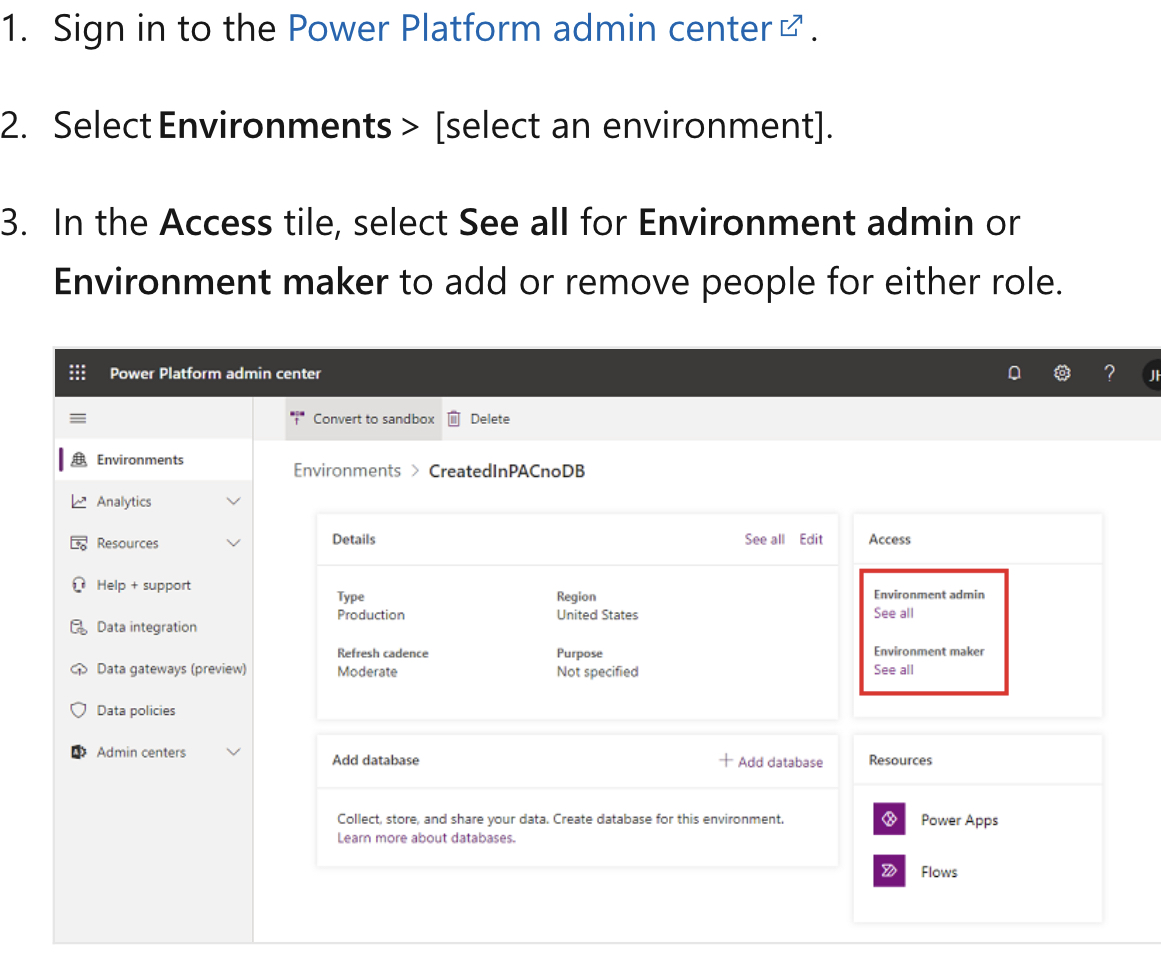
\includegraphics[scale = 0.3]{attachment/chapter_13/Scc011}
\end{figure}
Unter der Auswahl können dann Namen oder Gruppen hinzugefügt werden.
\begin{figure}[H]
	\centering
	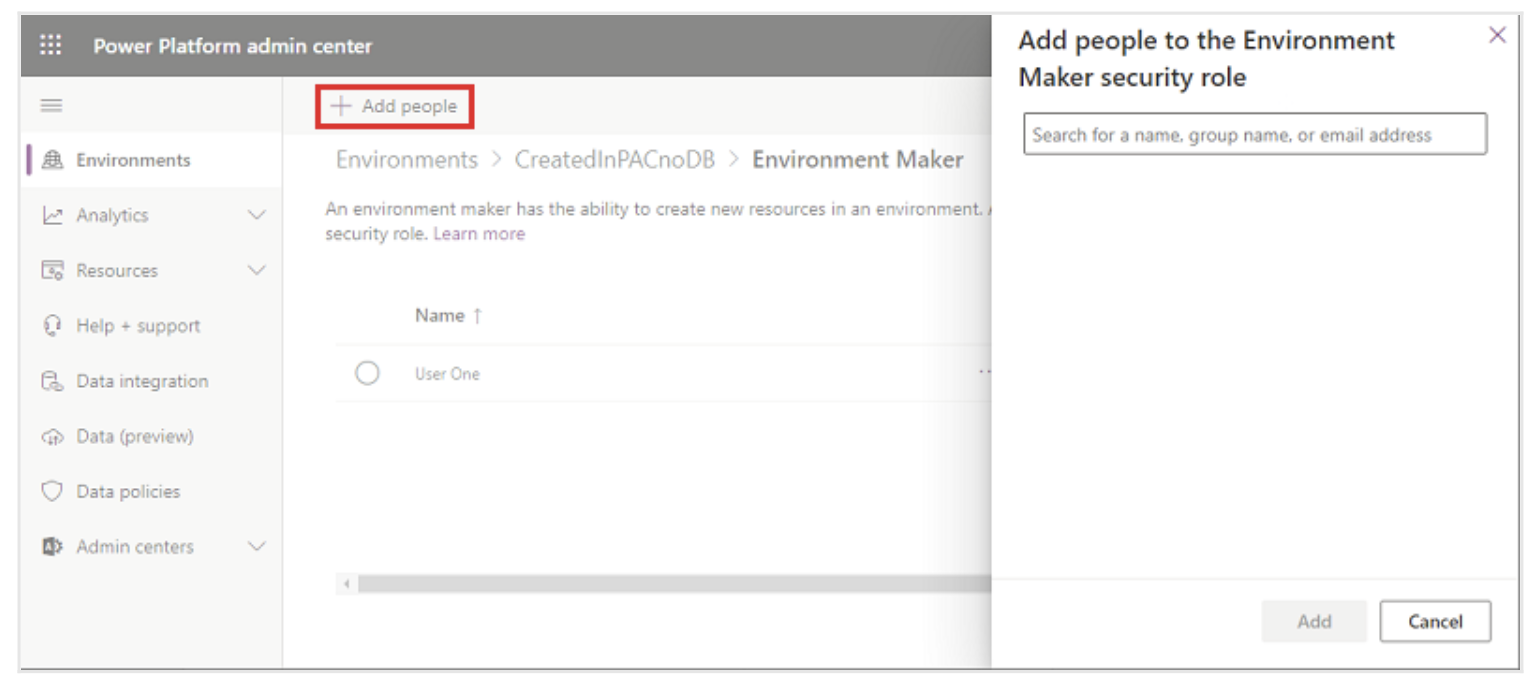
\includegraphics[scale = 0.3]{attachment/chapter_13/Scc012}
\end{figure}

\paragraph*{\Env mit CDS}
Sicherheitsrollen für \Env mit \gls{CDS} habe eine Erweiterung. Dies werden über \textit{Access/Security roles} gemanaget.
\begin{figure}[H]
	\centering
	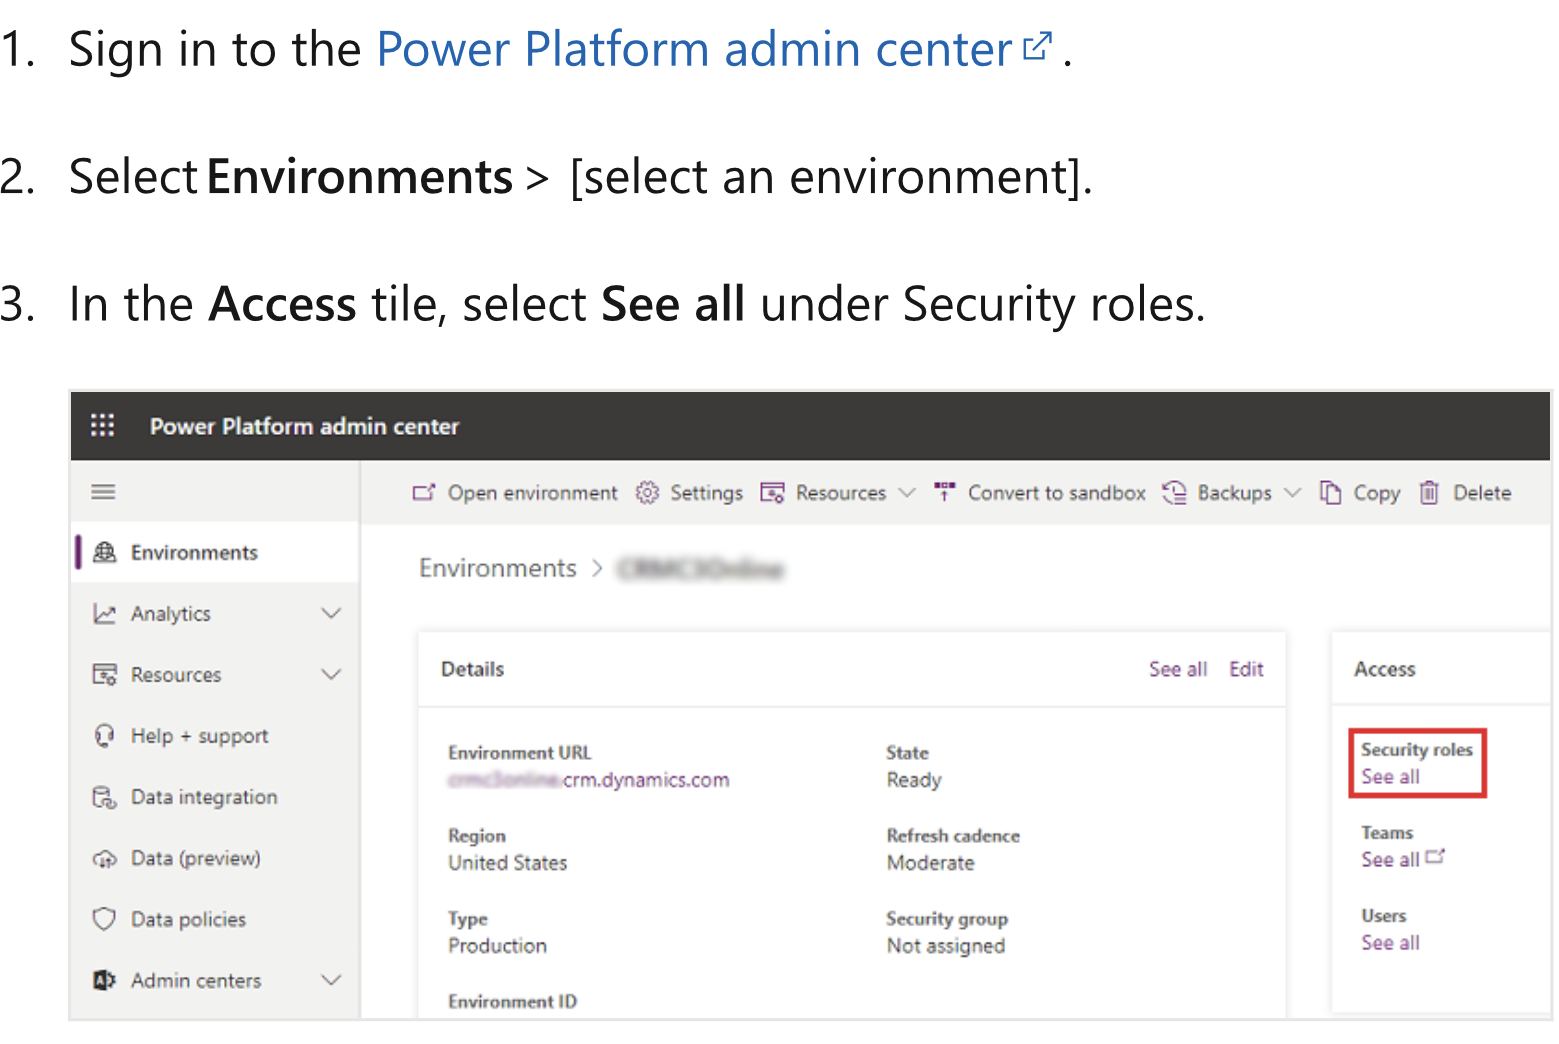
\includegraphics[scale = 0.3]{attachment/chapter_13/Scc013}
\end{figure}
Unter der Sicherheitsrolle gibt es die Auswahl \textit{Business unit}. Wenn diese ausgewählt ist, steht die List von vor und eigen definierten Sicherheitsrollen zur Verfügung.
\begin{figure}[H]
	\centering
	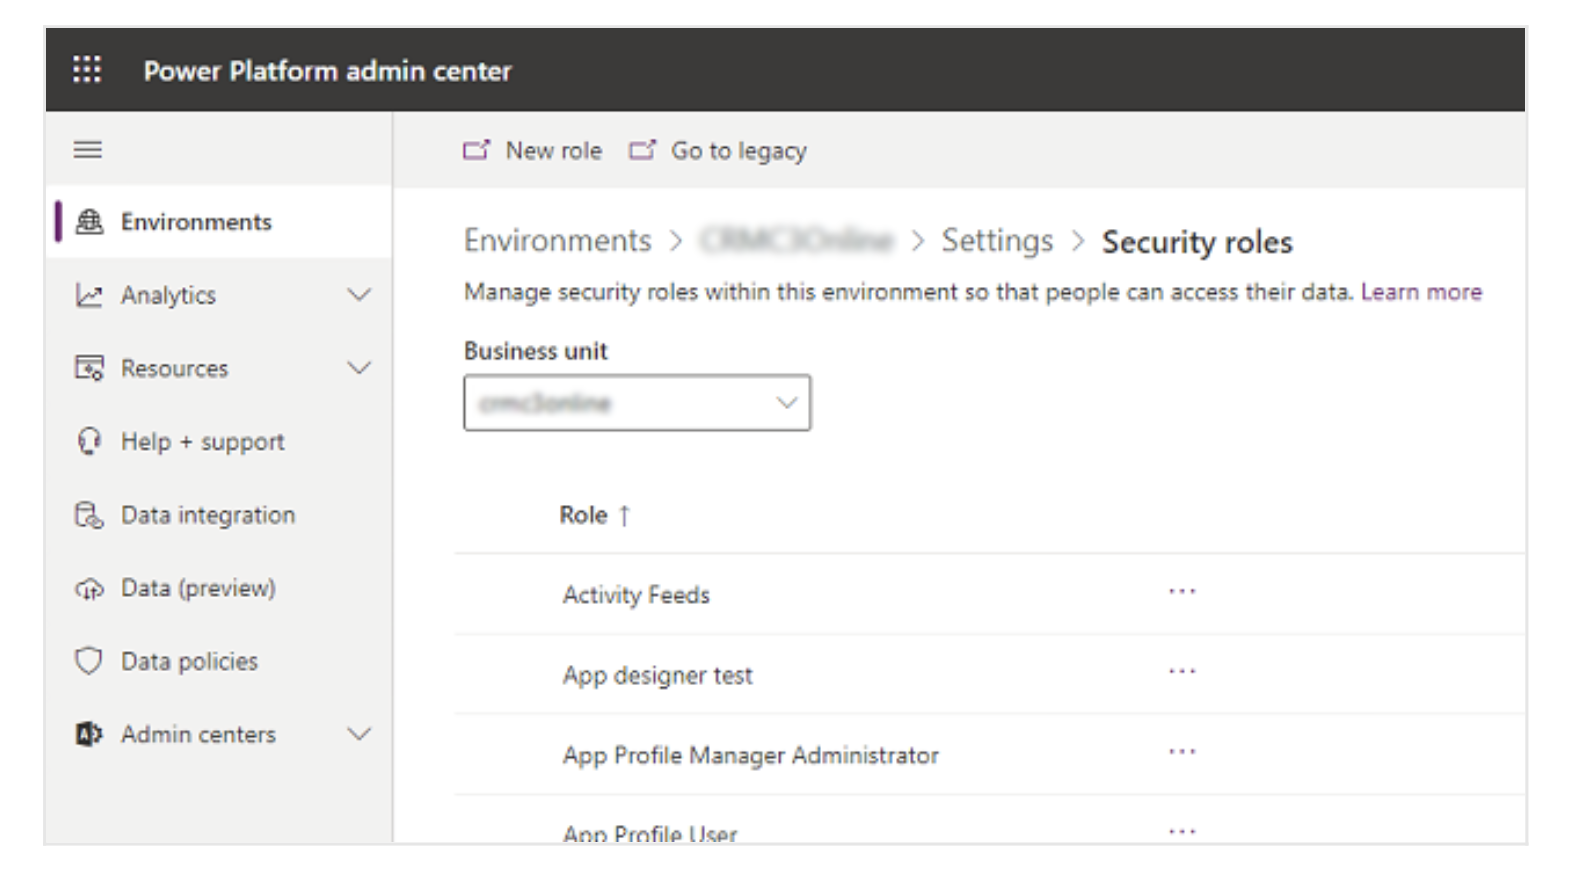
\includegraphics[scale = 0.3]{attachment/chapter_13/Scc014}
\end{figure}
Unter Auswahl der Business Unit und der Rolle kann wie gewohnt, eine Person oder Gruppe hinzugefügt werden.
\begin{figure}[H]
	\centering
	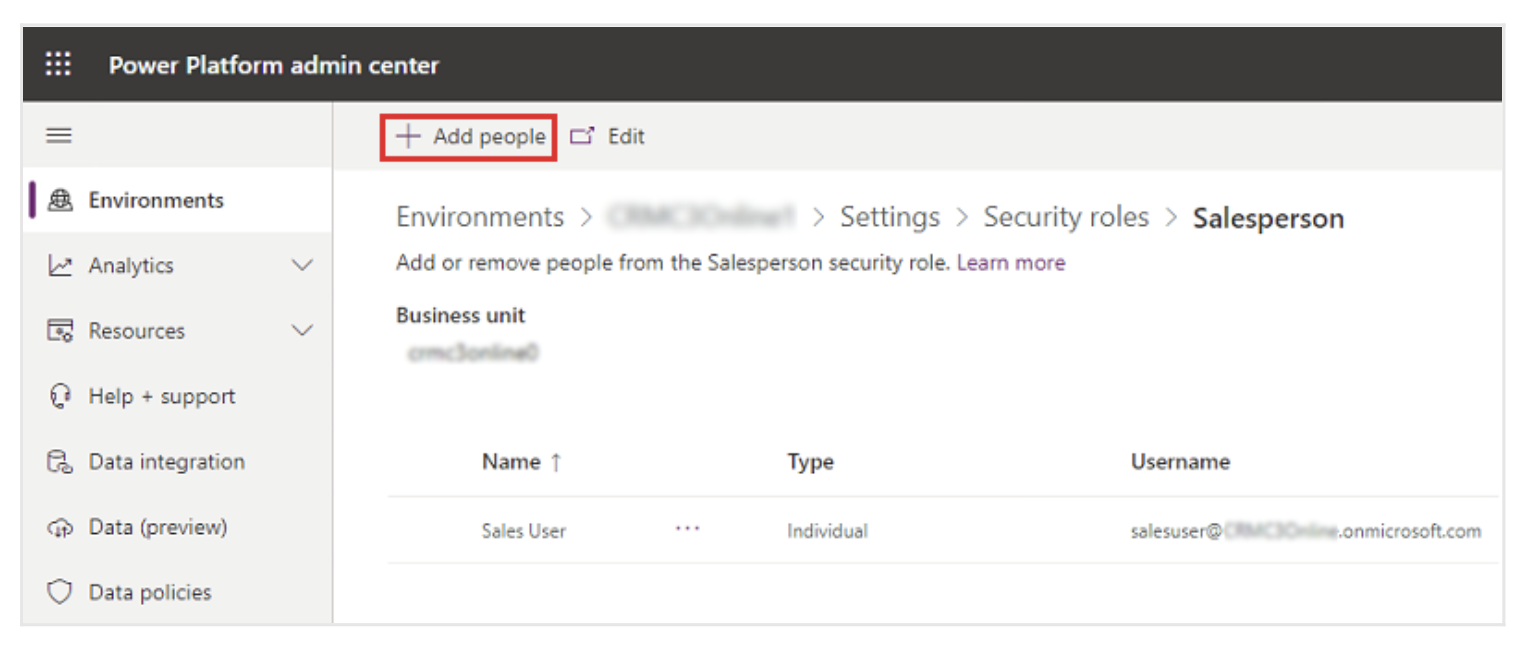
\includegraphics[scale = 0.3]{attachment/chapter_13/Scc015}
\end{figure}

\paragraph*{Custom Security Role}
Die Umgebung gibt eine URL an, welche unter Dynamics 365 das Advanced Admin Center erreicht.
\begin{figure}[H]
	\centering
	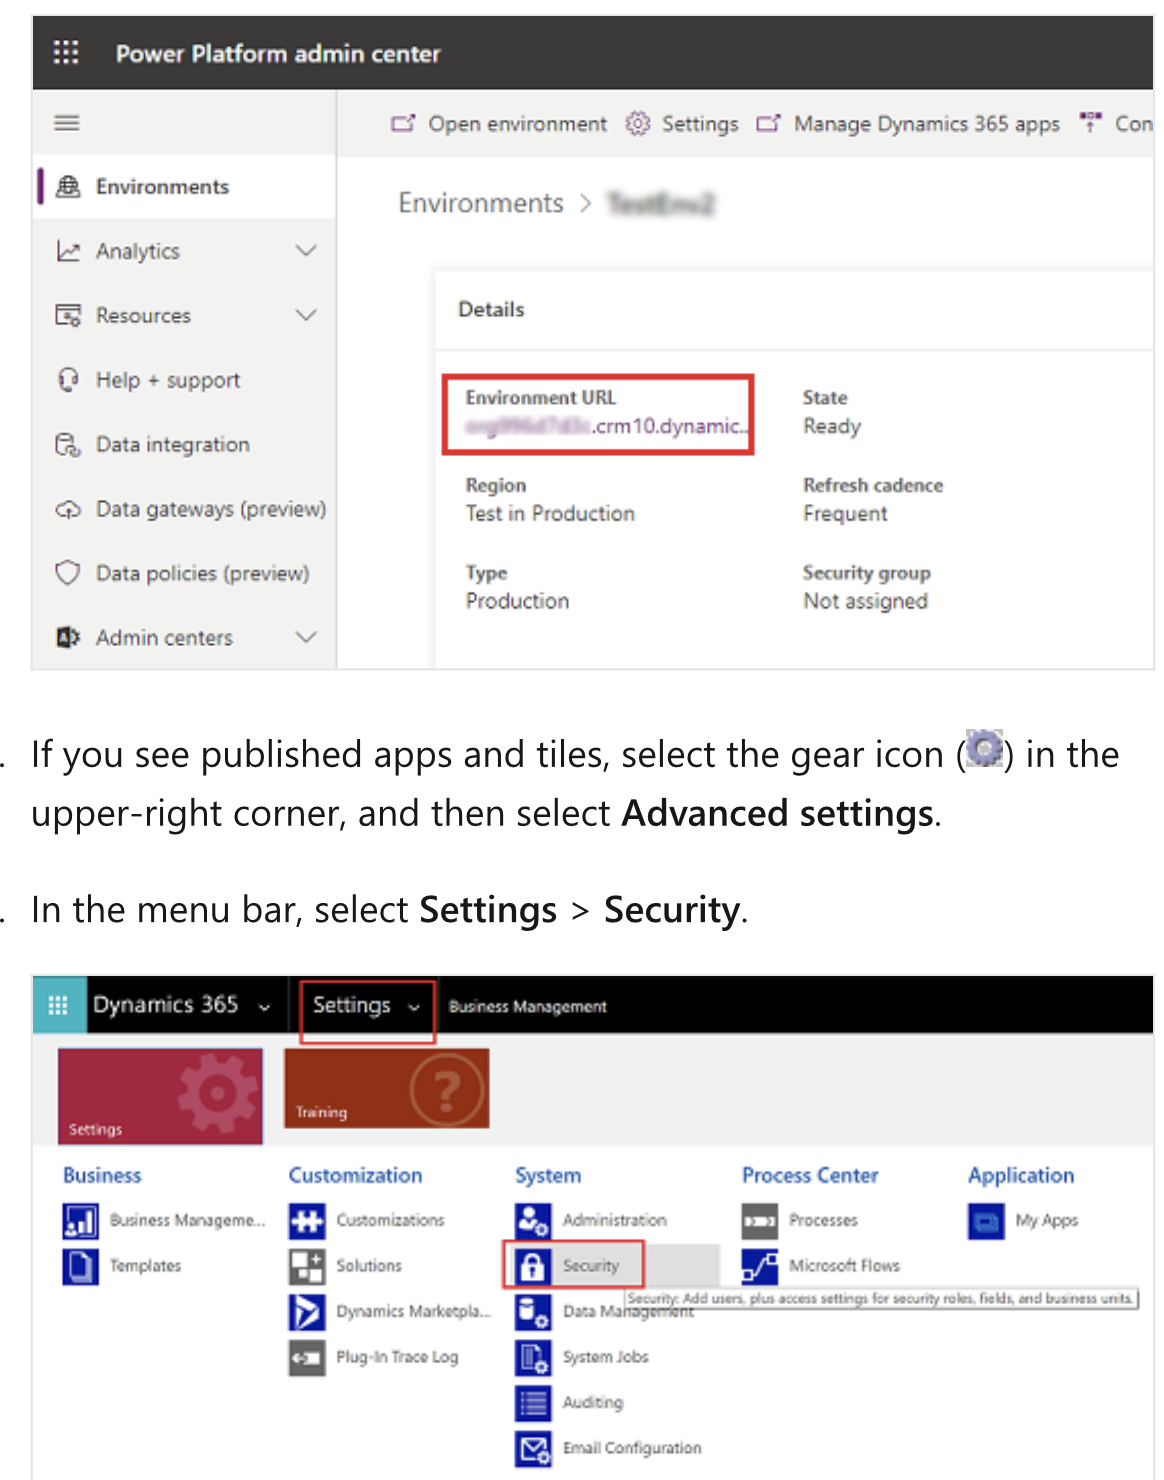
\includegraphics[scale = 0.3]{attachment/chapter_13/Scc016}
\end{figure}
Über diesen Bereich können neue Rollen angelegt werden. Unter \href{https://docs.microsof.com/en-us/power-platform/admin/database-security}{Security Roles} wird genau beschrieben, welche Mindestanforderungen eine neue Sicherheitsrolle haben muss. Die Hauptprivilegen sind \textit{lesen, schreiben und anfügen}.

\paragraph*{Different Types of Admin}
Der Globale Admin ist der Admin des Tenants.
\begin{figure}[H]
	\centering
	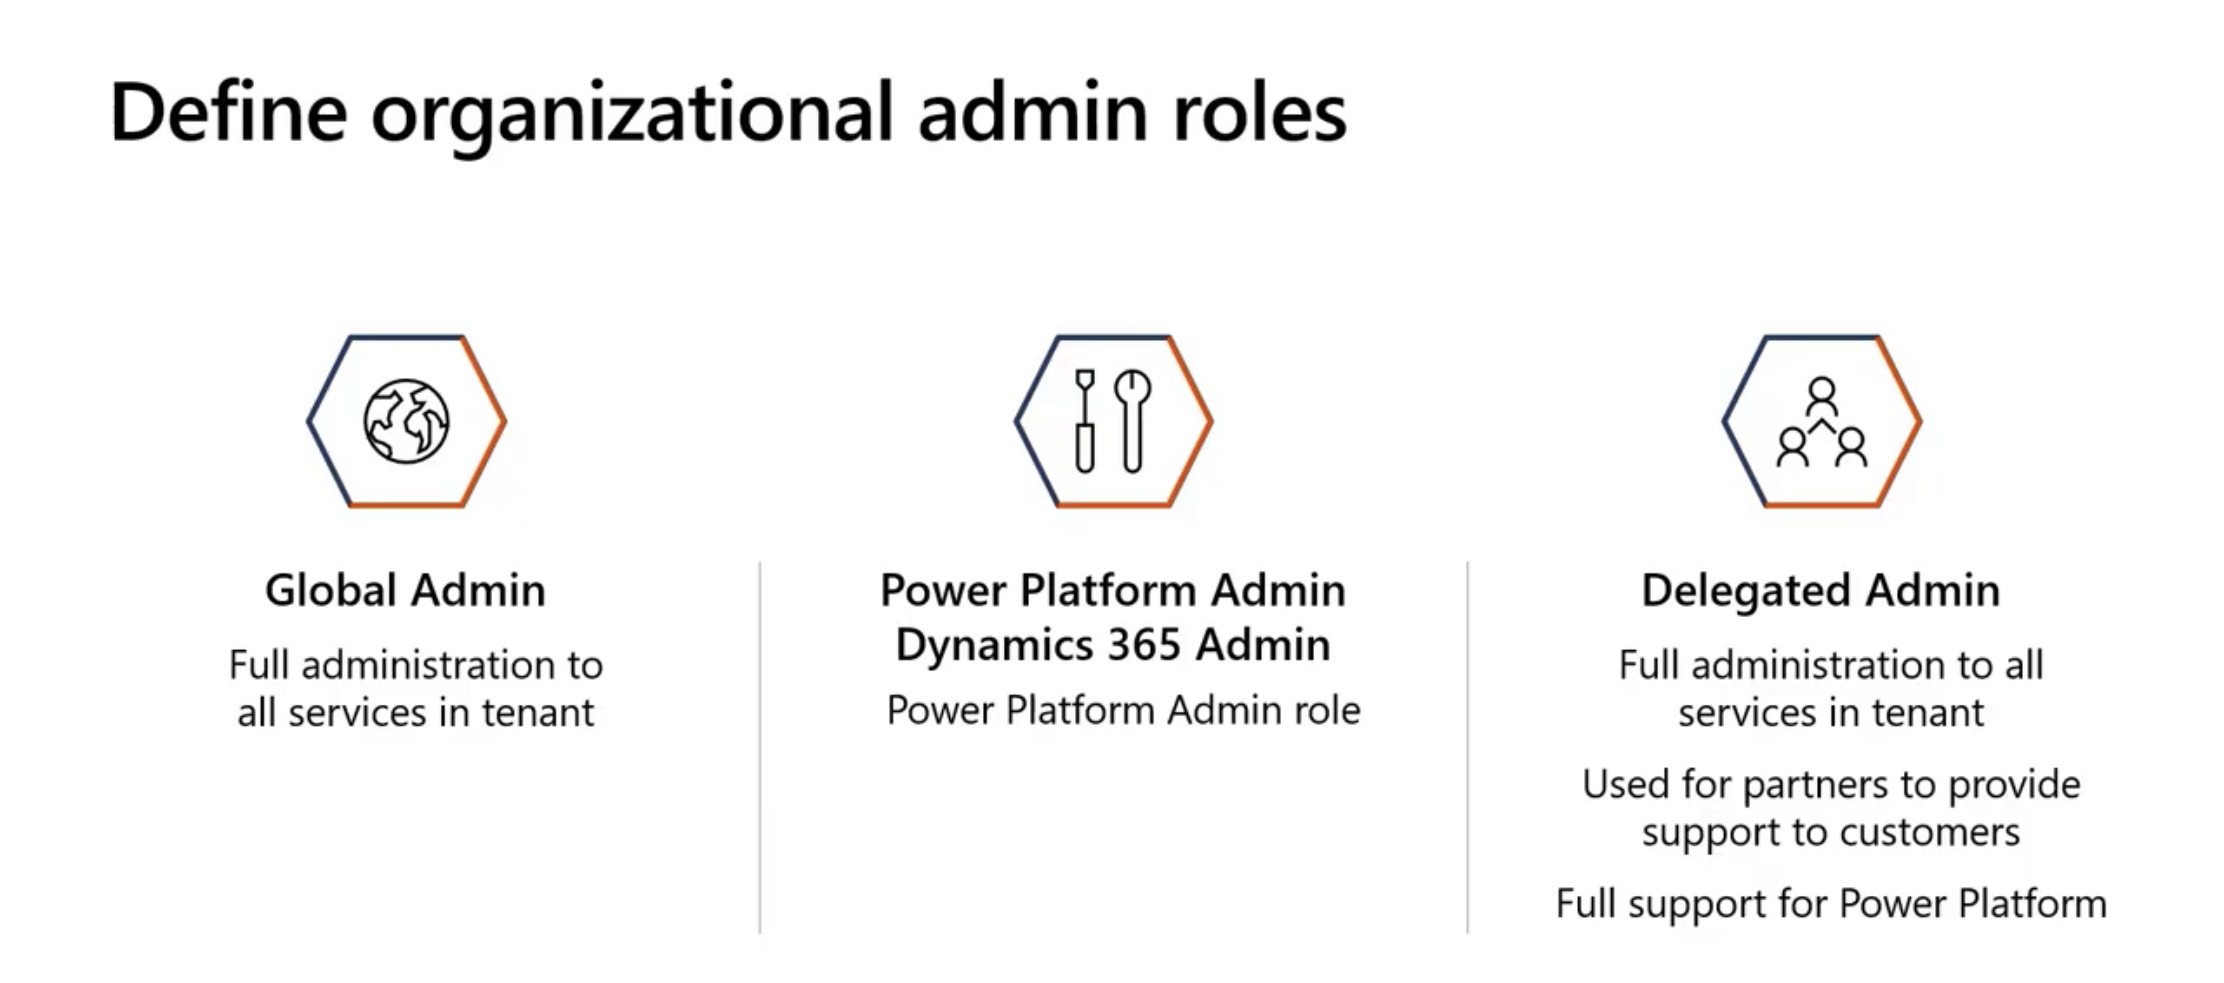
\includegraphics[scale = 0.3]{attachment/chapter_13/Scc001}
	\caption{Different admin roles in a organisation}
\end{figure}
\subsubsection{\Env}
\paragraph*{Default \Env}
Die \gls{PP} ist auf Microsoft Azure aufgebaut. Die Verwaltung (Azure AD), der Speicher (Storage) und weitere Komponenten sind Teil des Fundaments.
\begin{figure}[H]
	\centering
	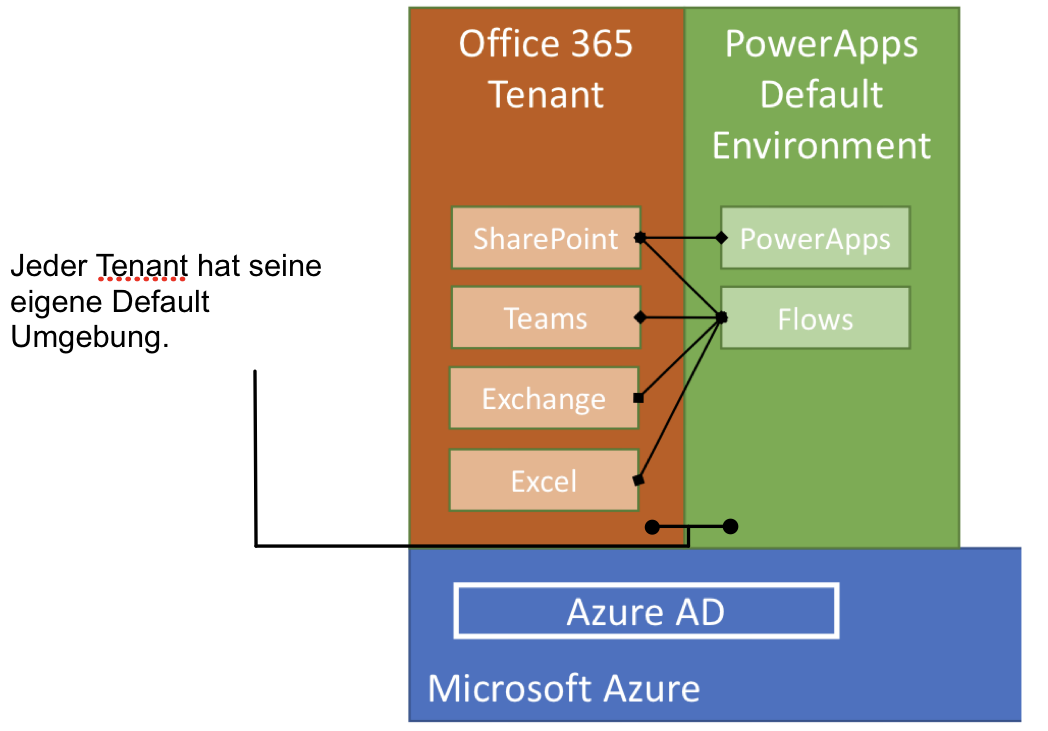
\includegraphics[scale = 0.3]{attachment/chapter_13/Scc008}
\end{figure}
Jeder Office 365 Tenant, meist für eine Organisation ist dies ein Tenant, erhält eine Default \Env für alle Nutzer. In diese Umgebung hat die \gls{PP} Default Umgebung über Power Apps Zugriff auf SharePoint und Flow kann sich zu den gängigen gional nächsten zur Azure AD des Tenents. Die Default kostenlose Kapazität beträgt \SI{3}{\giga\byte} für Dataverse Database sowie Dateispeicher. \\

Für die Default Umgebung erhält jeder User die \textbf{\Env Maker/ Umgebungs-Hersteller} Berechtigung. User sind, welche eine \gls{PP} Lizenz erworben haben. Diese werden automatisch der Umgebung zu gewissen. 

\paragraph*{\Env with and without CDS}\label{par: \Env with and without CDS} 
Neue \Env können mit und ohne \gls{CDS} erstellt werden. 
\begin{figure}[H]
	\centering
	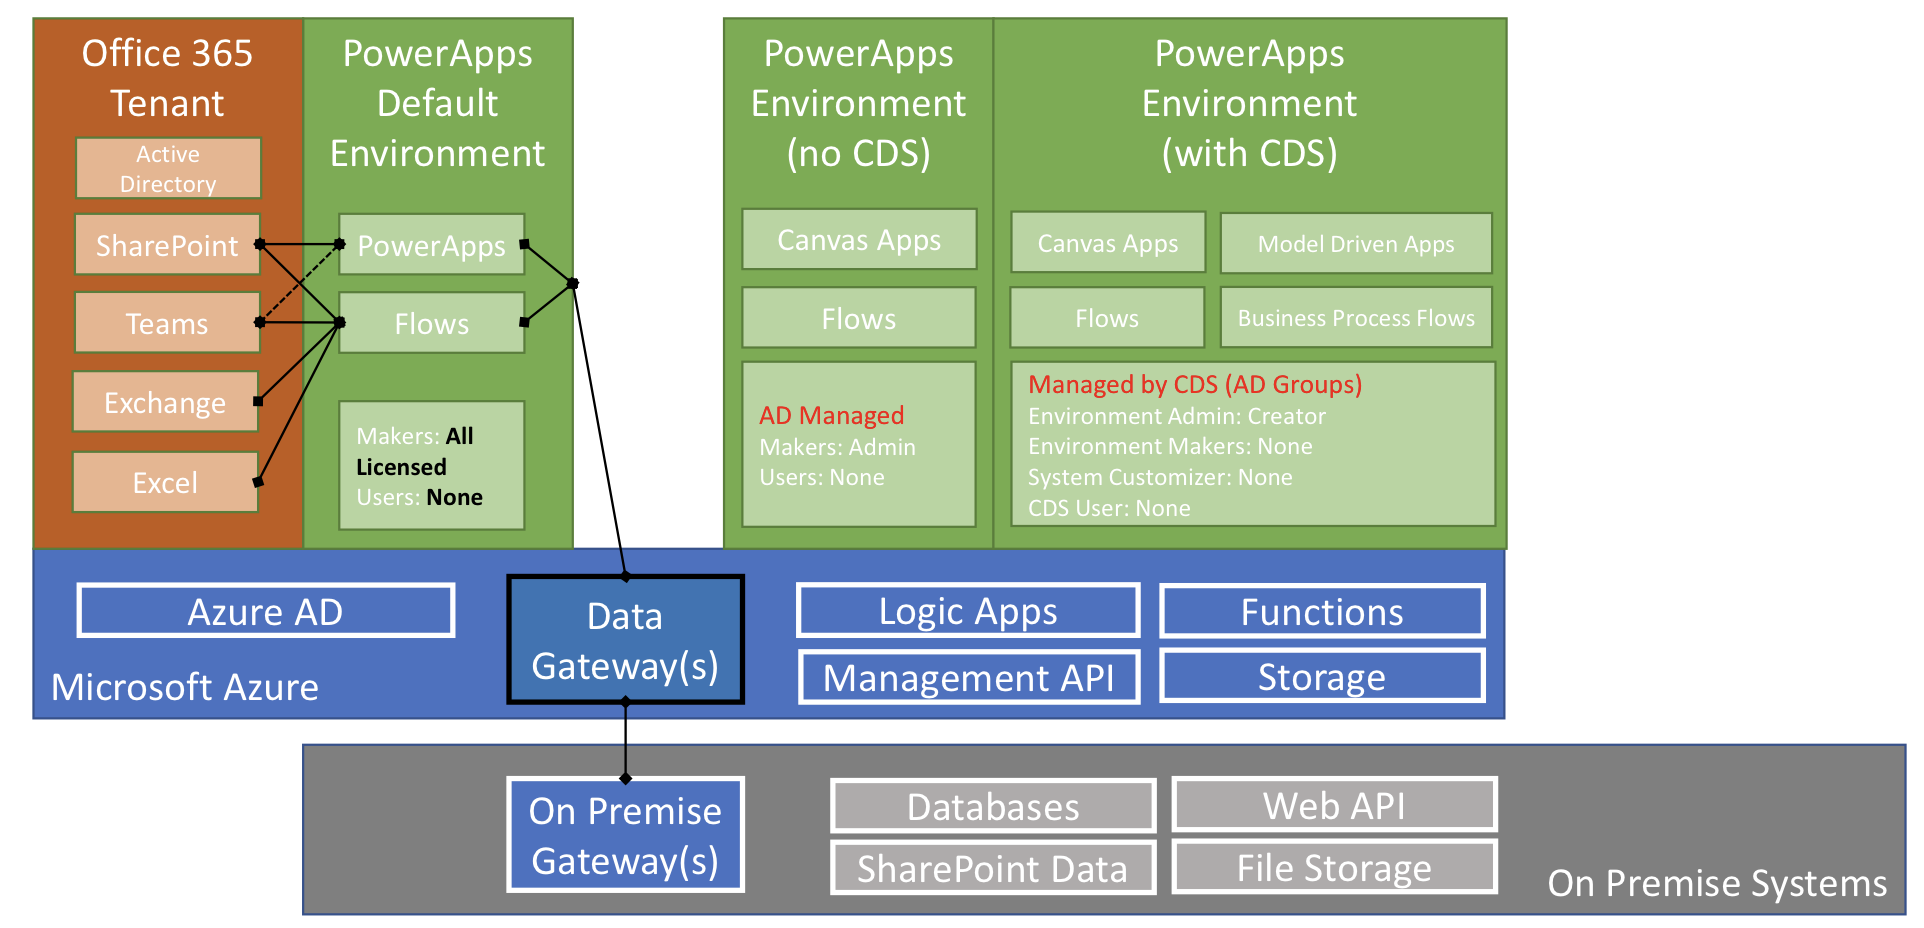
\includegraphics[scale = 0.3]{attachment/chapter_13/Scc009}
\end{figure}
In einer Umgebung ohne \gls{CDS} können nur Canvas Apps erstellt werden. Mit einer \gls{CDS} können Model-gestützt Apps erstellt werden.

\paragraph*{Typen von \Env}
Ein Umgebung kann verschiedenen Zwecke haben. Zur Auswahl stehen 6 Typen. Es gibt 3 bekannte Typen wie Produktion, Sandbox (Ursprünglich Develop) und Testing. Darüber hinaus gibt es noch diese haben besondere Funktionen und fall aus dem typischen Entwicklung-Testing-Deplop Prozess heraus.
\begin{description}
	\item[Production] Ist für die laufenden Arbeit in einer Organisation bestimmt. Es kann von einem Administrator oder eine Power Apps-Lizenz User erstellt werden. \textit{Security:} Vollzugriff
	\item[Sandbox] Die Umgebung ist für die Entwicklung und das Testen von Ressourcen gedacht. Um dies zu erleichtern, gibt es Funktionen wie Kopieren und Zurücksetzen. \textit{Security:} Für das Test in Ressourcen ist nur ein Nutzer-Zugriff nötig. Um Ressourcen zu bearbeiten und erstellen ist für die Entwickler eine \Env Maker Rolle notwendig. Die Erstellung von Sandbox kann unterdrückt werden. Die Umwandlung einer Sandbox in Produktion ist möglich.
		\item[Trial/ Testing*] Ist für kurzfristiges Test vorgesehen. Diese werden nach 30 Tage wieder entleert. Jeder Nutzer kann nur eine Umgebung erstellen. Zweck diese ist, Proof-of-Concepts zu erstellen. \textit{Security:} Die Erstellung kann durch den Admin blockiert werden. Diese können einstellen, dass nur Tenat Admin Trial \Env erstellen können oder jeder im Tenant Bereich.
	\item[Default/Standard*] Dies wird für jeden Tenant/ Mandanten erstellt. Jeder lizensierte User wird dieser Umgebung mit der \Env Maker Rolle zugewiesen. \textit{Security:} Limitierter Zugriff.
	\item[Develop*] Diese Umgebung kann nur von Nutzer erstellt werden, die einen Power Apps Develop Plan haben. Eine Erstellung dieser Umgebung kann nicht blockiert werden, wenn ein Nutzer die entsprechende Lizenz hat, außer durch ein Support Ticket. \textit{Security:} Ersteller können weitere Nutzer als \Env Maker hinzufügen. 
	\item[Dataverse Microsoft Teams*] Ist für das Erstellen von Power Apps aus einem Team heraus vorgesehen. Ein Dataverse wird automatisch erstellt, wenn eine App erstellt oder aus einem Katalog über Teams ausgewählt wird. \textit{Security:} Eingeschränkt Möglichkeiten. Nutzer aus dem Team werden automatischen ihrer Rolle im Dataverse mit einer Sicherheitslevel ausgestattet. Änderungen sind nicht möglich. 
\end{description}

Welcher Typ die Umgebung besitzt kann in der Auflistung eingesehen werden.
\begin{figure}[H]
	\centering
	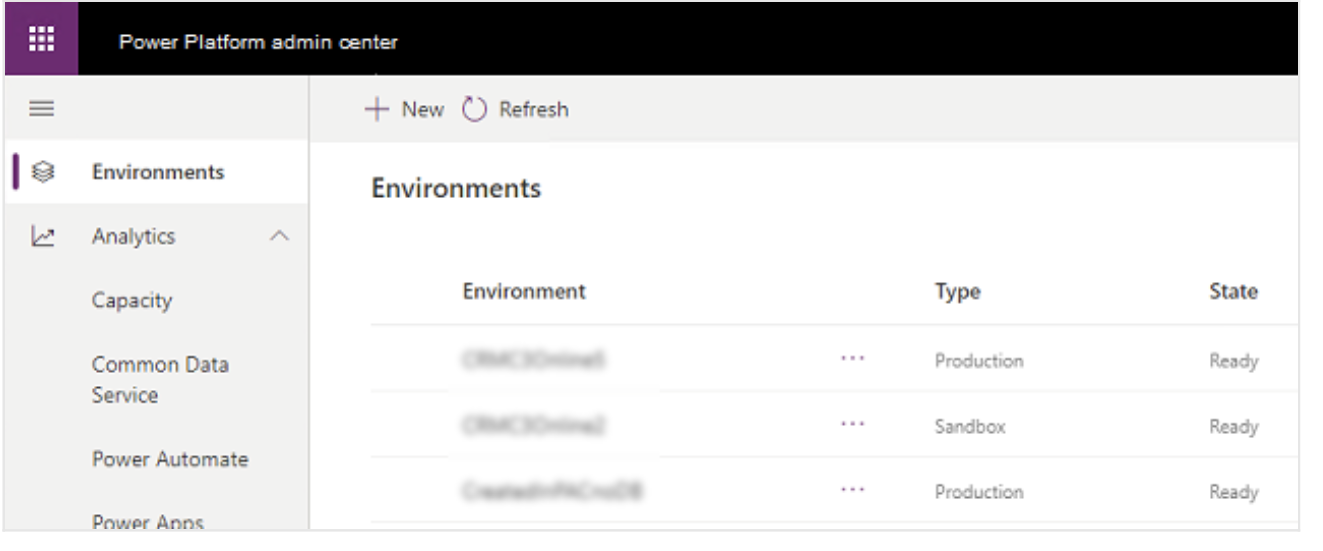
\includegraphics[scale = 0.3]{attachment/chapter_13/Scc017}
\end{figure}

\paragraph*{Create \Env}
Wenn eine Umgebung mit einer Datenbank erstellt wird, muss wie oben erwähnt werden, der Type der Umgebung spezifiziert werden und unten die Option, ob diese Umgebung mit einer Datenbank erstellt wird, auf Ja gesetzt werden.
\begin{figure}[H]
	\centering
	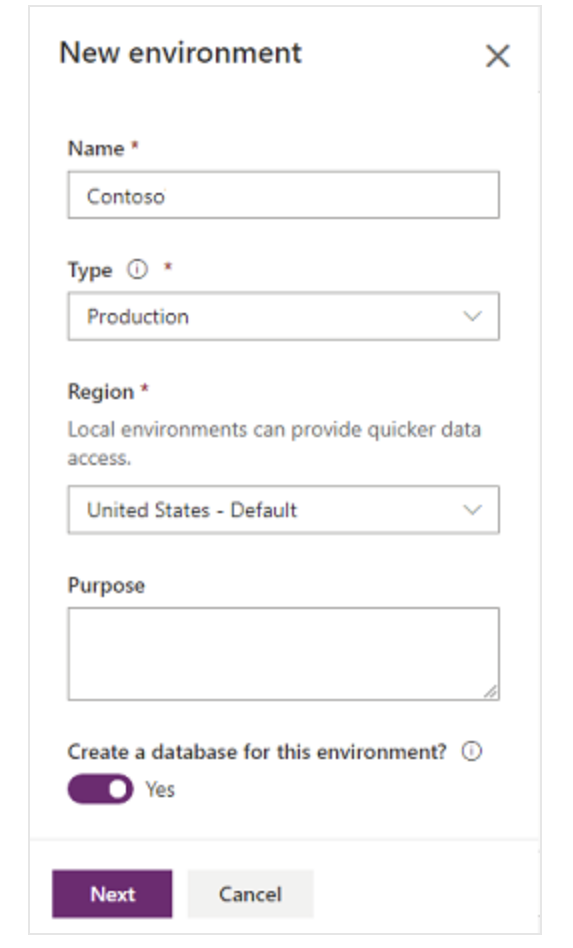
\includegraphics[scale = 0.3]{attachment/chapter_13/Scc018}
\end{figure}
Für die Datenbank wird die Erweiterung benötigt, 
\begin{itemize}
	\item welche Sprache für die Umgebung gilt,
	\item wie die Firmen URL ist. Im Fall der \gls{DB} ist es \textit{dbsw},
	\item Erweiterung für Dynamics 365 und 
	\item Sicherheitsgruppe. Wenn diese nicht angegeben wird, kann jeder unter dem Tenant die Umgebung sehen.
\end{itemize}
\begin{figure}[H]
	\centering
	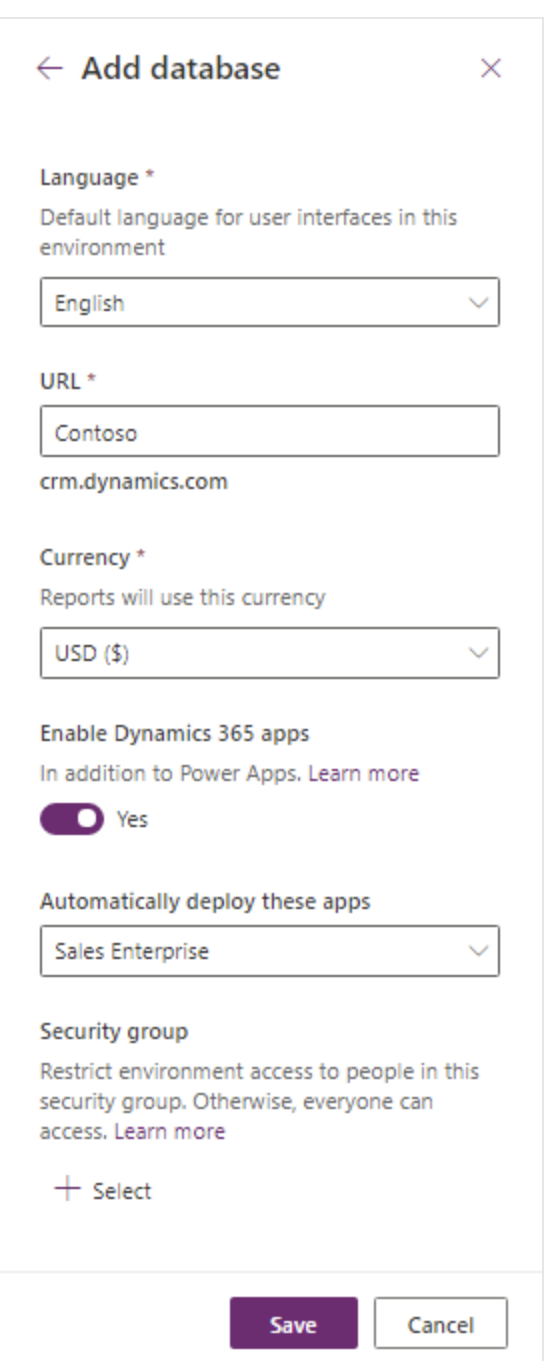
\includegraphics[scale = 0.3]{attachment/chapter_13/Scc019}
\end{figure}
Ebenso ist es möglich eine Umgebung zu erstellen, welche ohne ein Dataverse erstellt wird.

Für Admins ist es möglich die Erstellung von \Env zu unterdrücken. Diese können unter \textit{admin.powerplatform.microsoft.com} auf Setting (nur für Admins einsehbar), die Einstellung
\begin{figure}[H]
	\centering
	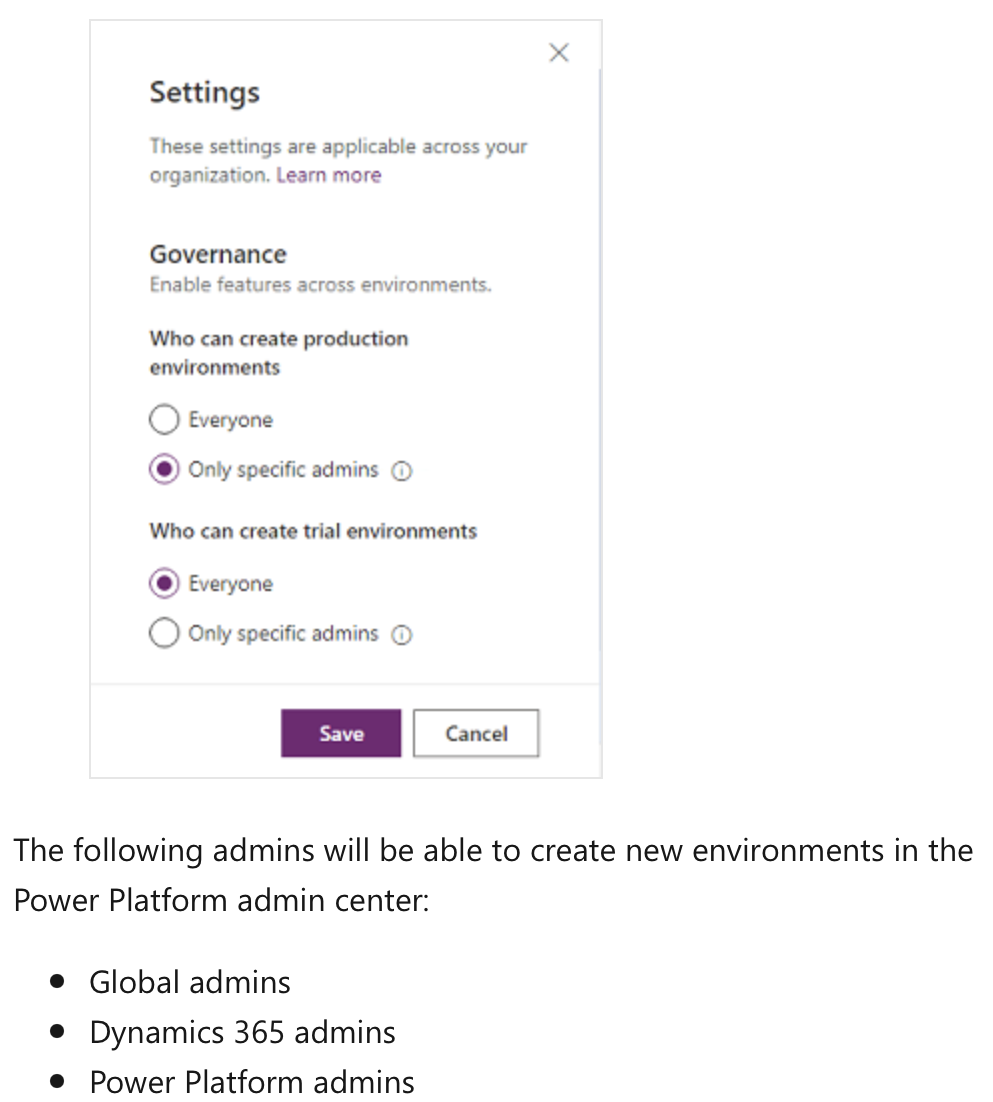
\includegraphics[scale = 0.3]{attachment/chapter_13/Scc020}
\end{figure}
auf \textit{only Admins} setzen. Als Admins werden 
\begin{itemize}
	\item Global Admin,
	\item Dynamics 365 Admin und
	\item \gls{PP}Adin
\end{itemize}
verstanden. Diese können \Env erstellen. \footnote{Für die Kontrolle dieser Umgebung, kann \textit{PowerShell cmdlets} heruntergeladen werden, sodass die Einstellung über die Comando Zeile erfolgt. \begin{figure}[H]
		\centering
		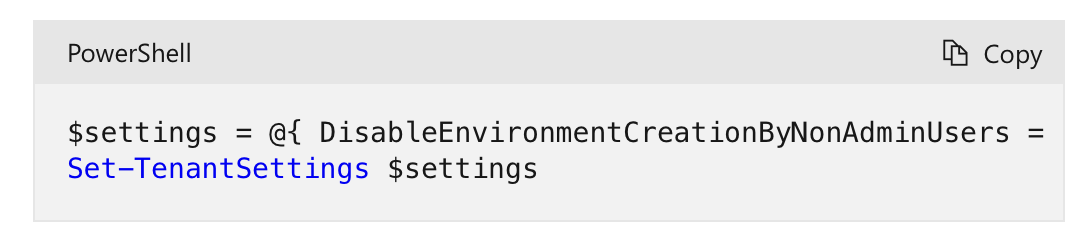
\includegraphics[scale = 0.3]{attachment/chapter_13/Scc021}
\end{figure}}

Für Sandbox \Env gilt, dass dies auch wieder reset werden können. Dies bedeutet, dass die Umgebung erhalten bleibt, aber alle Komponenten gelöscht werden.

\paragraph*{Convert \Env Type}
 Neben dem Zyklus von Enwicklung-Test-Produktion können die \Env Produktion und Sandbox auch ihren Type ändern. Dabei werden die \Env konvertiert. Dies geht nur in der Administrator Rolle.
\begin{figure}[H]
	\centering
	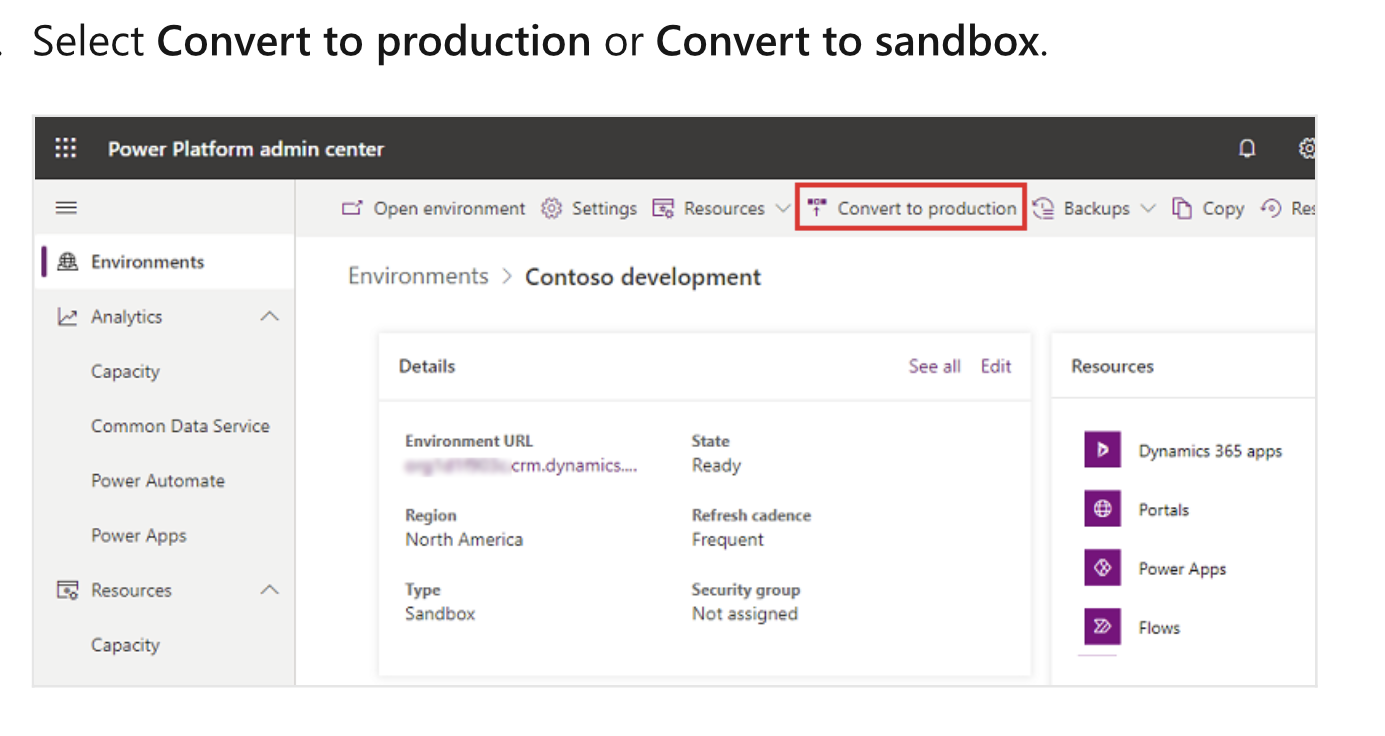
\includegraphics[scale = 0.3]{attachment/chapter_13/Scc022}
\end{figure}
Es ist möglich \textit{Sandbox} in \textit{Produktion} umzuwandeln oder umgekehrt.
Dieser Prozess kann einige Stunden dauern.
\begin{figure}[H]
	\centering
	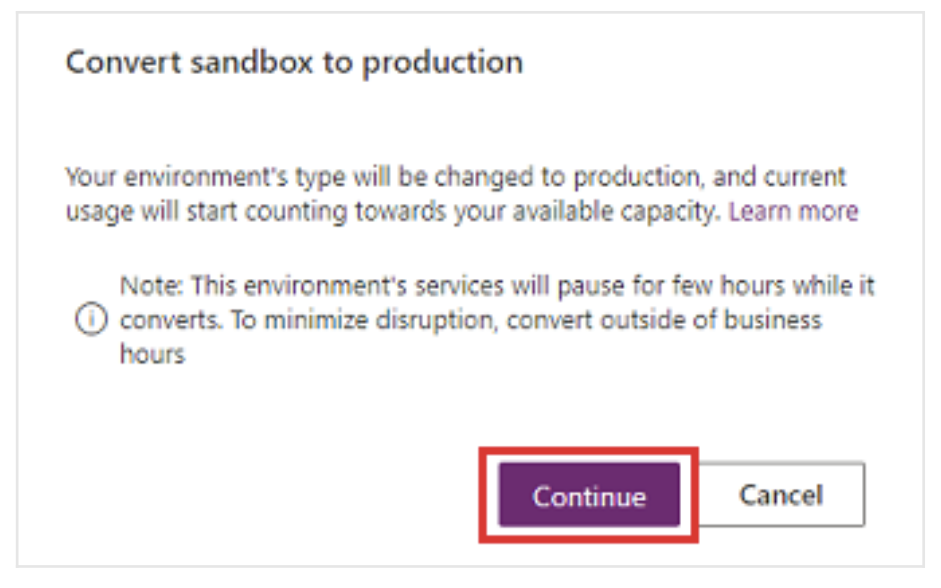
\includegraphics[scale = 0.3]{attachment/chapter_13/Scc023}
\end{figure}

\paragraph*{Adding a Database}
Wurde eine Umgebung erstellt, in welcher keine Datenbank (Dataverse) erstellt wurde, kann dies auf zwei Arten erfolgen:
\begin{itemize}
	\item Detailseite der Umgebung oder
	\item Daten Panal/ Enties	
\end{itemize}
Auf der Hauptseite der Umgebung ist der Button \textit{Add database} zu sehen. Diese ist nur für Admins mit der entsprechenden Lizenz zu nutzen. Wenn darauf geklickt wird, müssen die Details wie unter \refname{par: \Env with and without CDS} eingegeben werden. 

\begin{figure}[H]
	\centering
	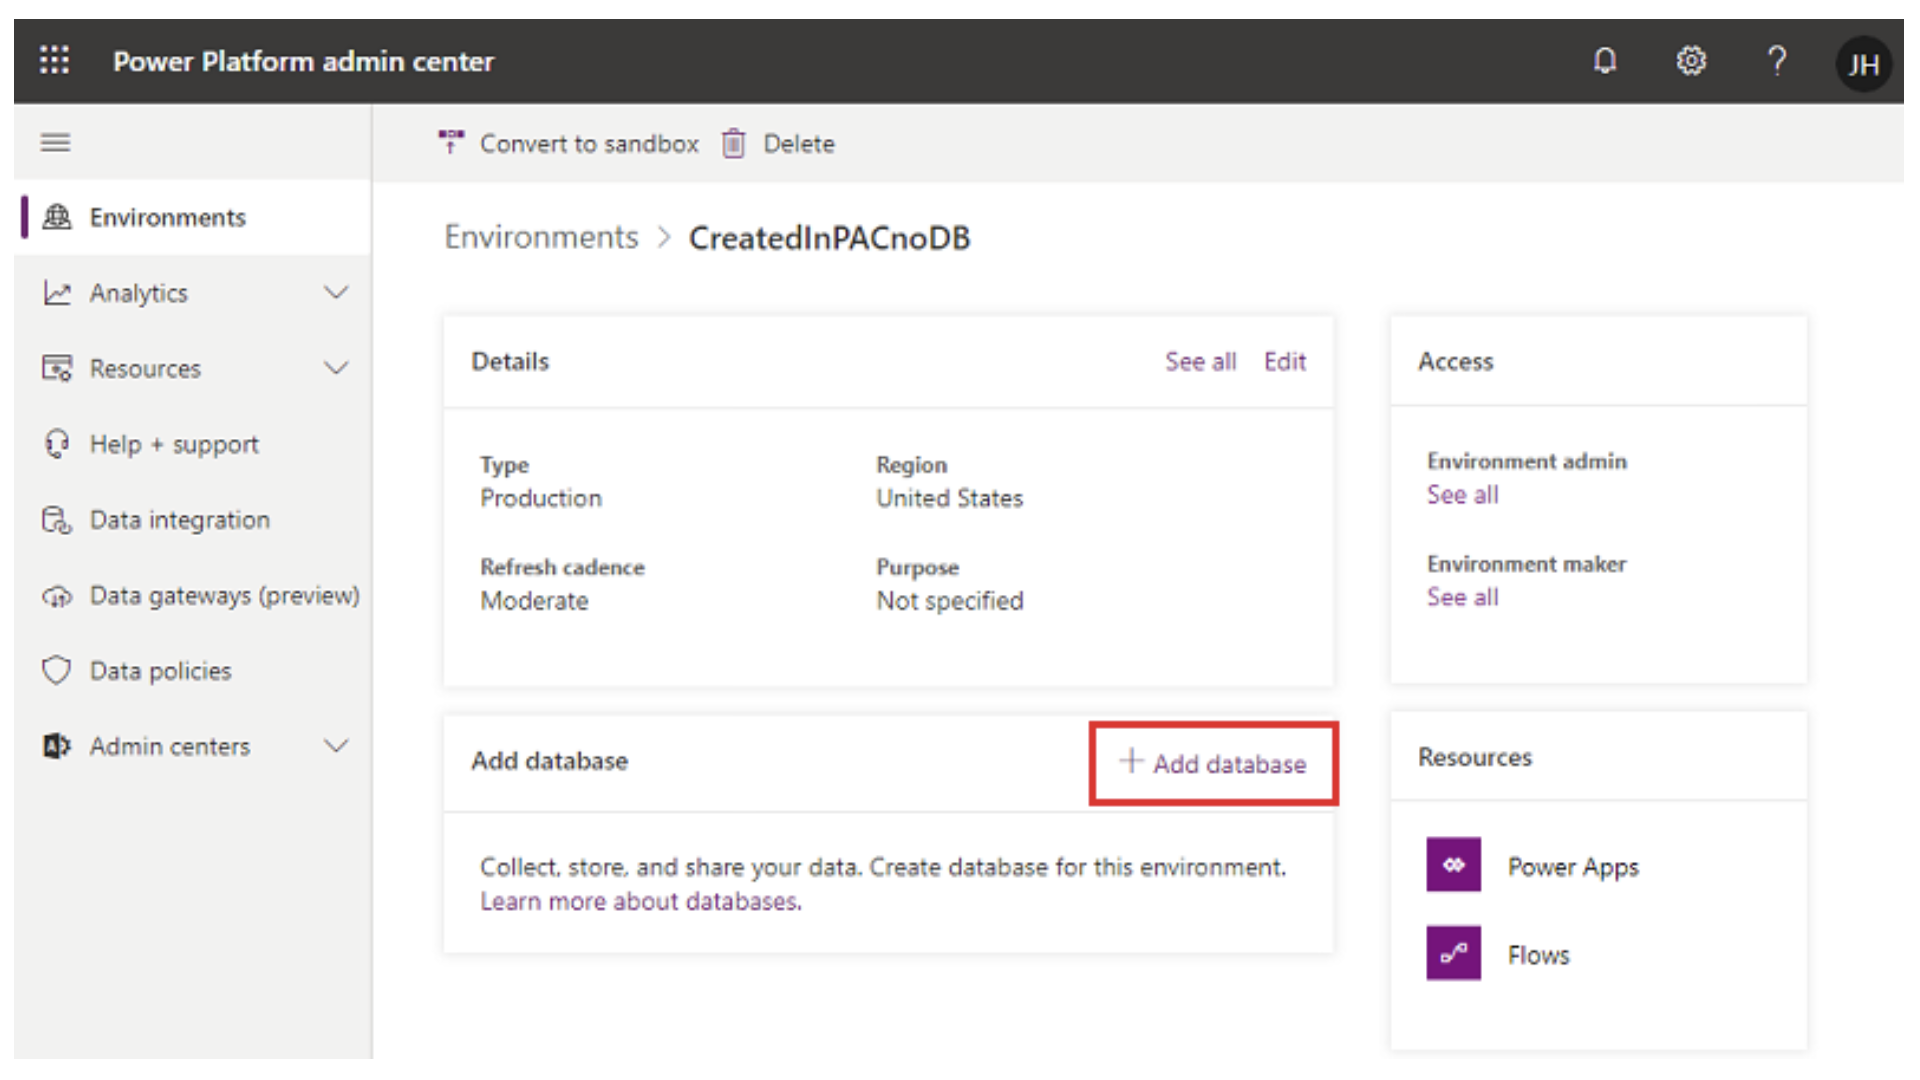
\includegraphics[scale = 0.3]{attachment/chapter_13/Scc024}
\end{figure}

Im zweite Option besteht unter in der \textit{Power Apps} Umgebung unter dem \textit{Daten Panal} ebenfalls eine Datenbank hinzuzufügen. 

\begin{figure}[H]
	\centering
	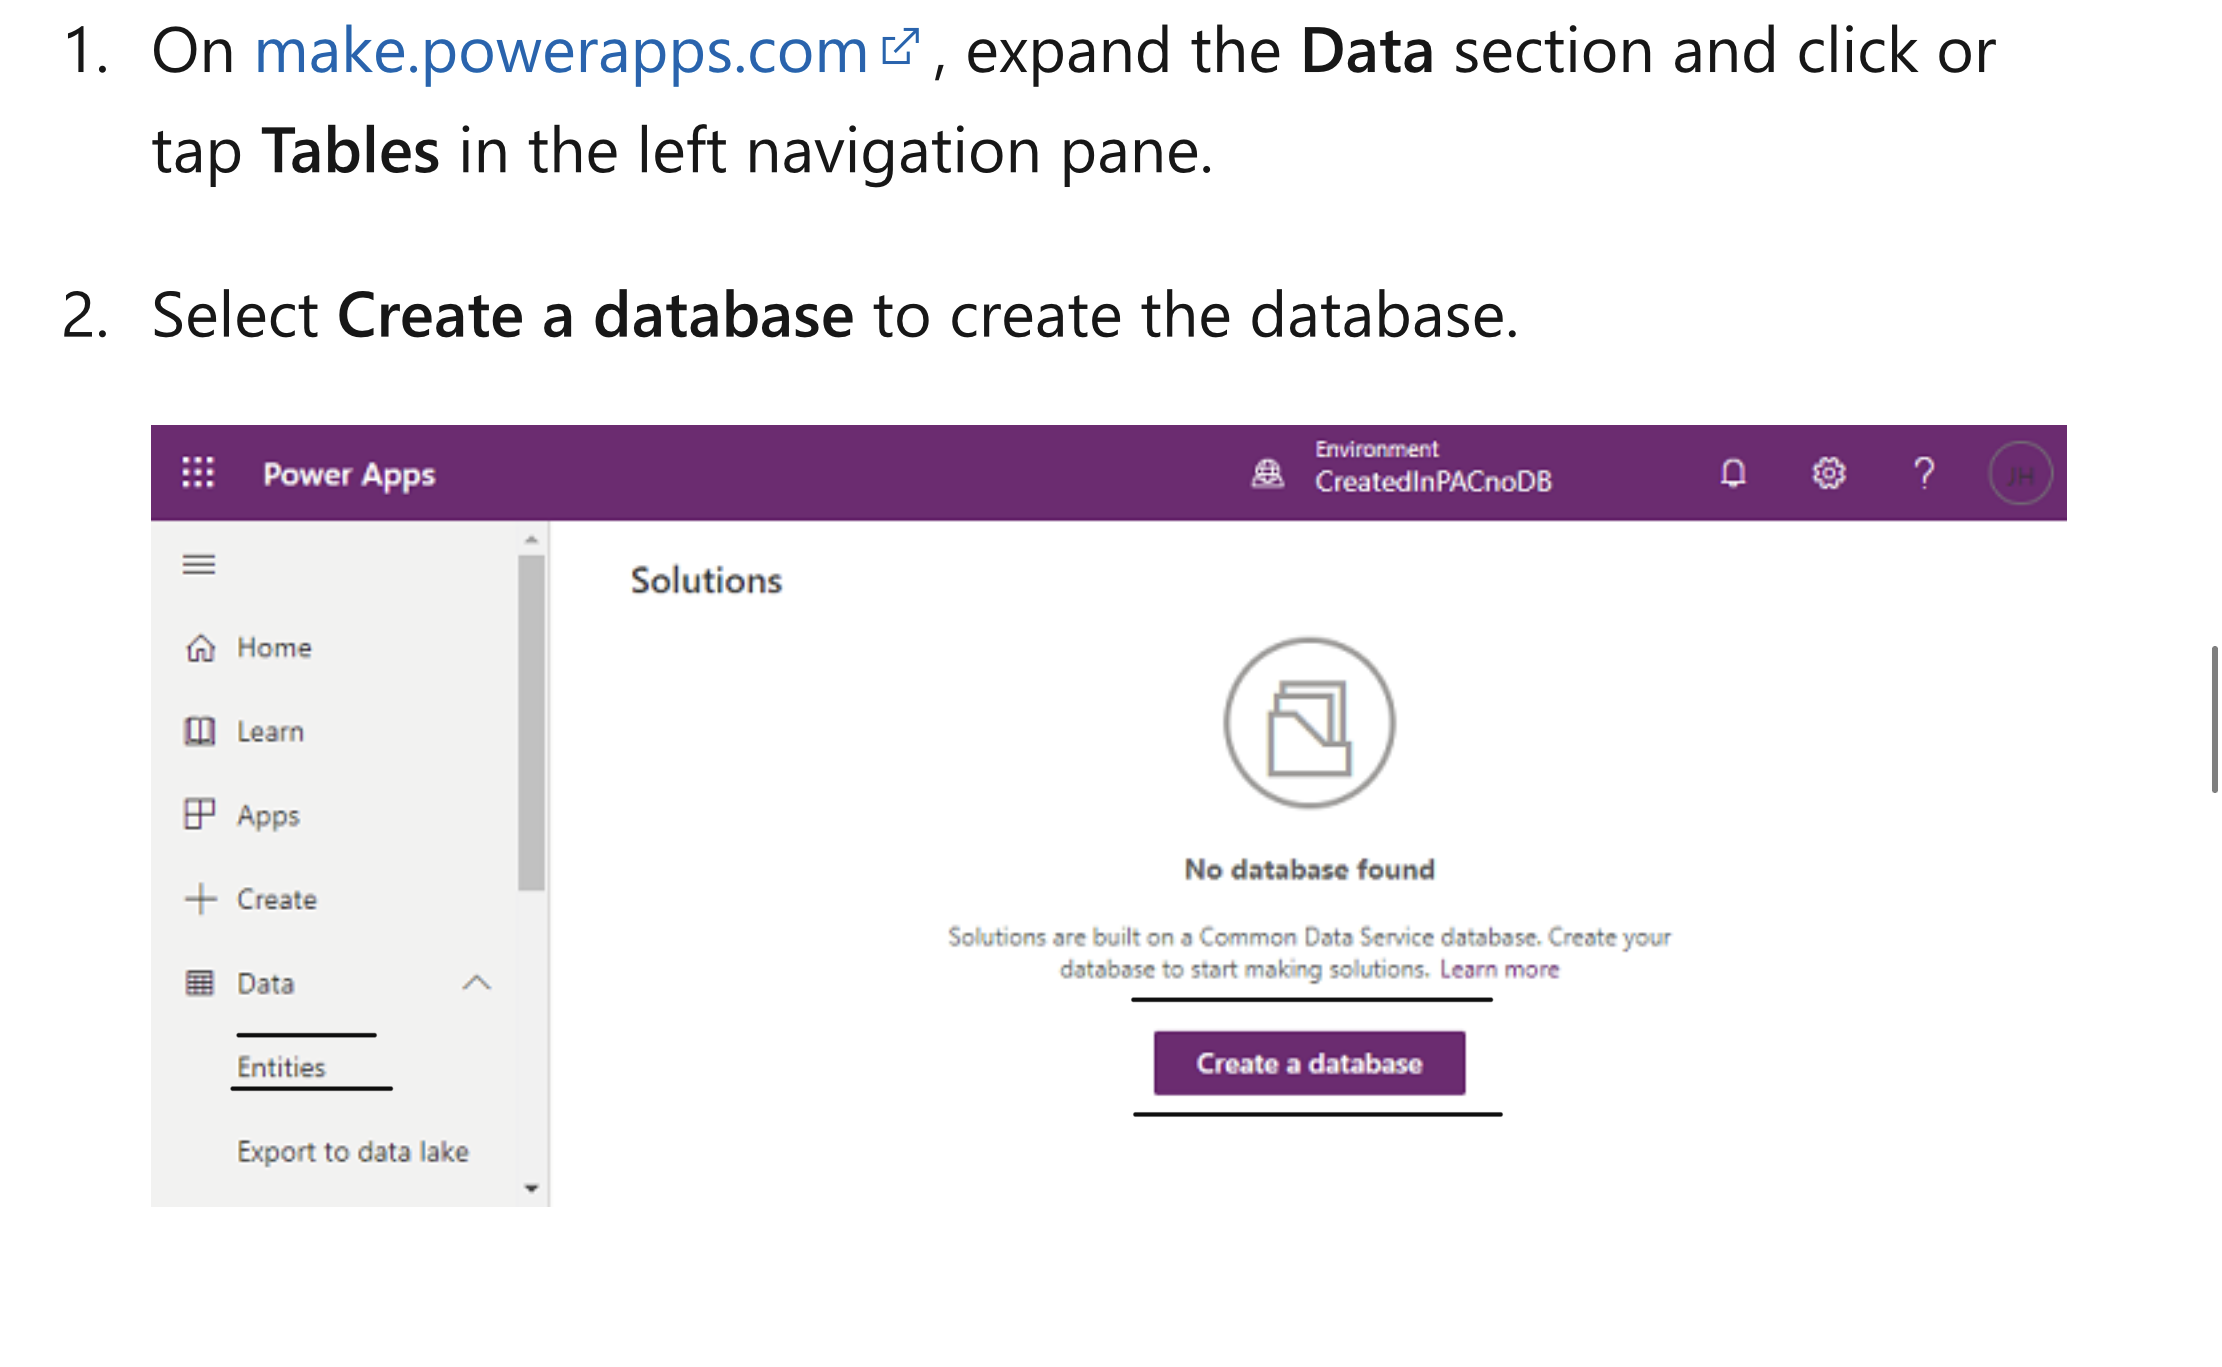
\includegraphics[scale = 0.3]{attachment/chapter_13/Scc025}
\end{figure}

\paragraph*{Copy \Env}
Dieser Zweck ist noch unklar.

\paragraph*{Administration Mode}
Über die Einstellung einer Umgebung kann eine Umgebung (Sandbox, Trial, Produktion) in den Administrierten Modus gesetzt werden. Ist dies geschehen, können nur noch System Admins in die Umgebung sich einwählen. Hinweis. Wenn der Modus wieder aus dem Admin Modus genommen wird, kann es bis zu 24 Stunden dauern kann, bis alle Flows wieder aktiv sind.


\subsection{Lizenzstruktur}
\paragraph{DB Lizenzen}
Im Folgenden wird die Lizenzstruktur am Beispiel des DB Konzern aufgezeigt.

Die angebotenen Lizenzen sind
\begin{itemize}
	\item Power Automate $\&$ Apps Basic,
	\item Power Apps Full User,
	\item Power Automate Full User,
	\item Power Apps DualApp Packet und
	\item die Power Automate Flow Lizenz.
\end{itemize}

Die Betrachtung, welche Lizenzen benötigt werden, werden mehrer Kategorien betrachtet werden:
\begin{itemize}
	\item Konnektoren,
	\item \gls{API} Abfragen,
	\item Anwendungsfall: Automate, Apps oder beides
	\item Vier DB-Nutzergruppen
		\begin{itemize}
			\item User (Benutzer)
			\item Developtment-Verwandtwortliche (Anwendungsverantwortlicher)
			\item Entwickler (Anwendungsentwickler)
			\item 
		\end{itemize} 
\end{itemize}

Themen Referenzen: \href{https://docs.microsoft.com/de-de/power-platform/admin/power-automate-licensing/types}{Lizenz Typen}

\paragraph{Konnektoren}
Bei der Betrachtung wird ebenfalls unterschieden, welcher Anwendungsfall berücksichtig wird, Automate, Apps oder beides.

\section{Application Lifecycle Management (ALM)} 

\subsection{Allgemein}
Der \gls{ALM} Prozess unterstützt bei der dem Zyklus der Low-Code Anwendungen der Power Platform. Die \gls{PP} bittet die Entwicklung von Apps in einer einfacheren Gestalt. Die Konzepte wie Qualitätskontrollen, Goverance und \gls{CI}/\gls{CD} werden unter dem Begriff \gls{ALM} zusammengefasst.\\

\begin{center}
	Die \gls{PP} und andere Anwendungen der Microsoft Umgebung helfen den Lebenzyklus von \gls{PP} Anwendungen in einer nachhaltigeren Weise umzusetzen.
\end{center}

\begin{figure}[H]
	\centering
	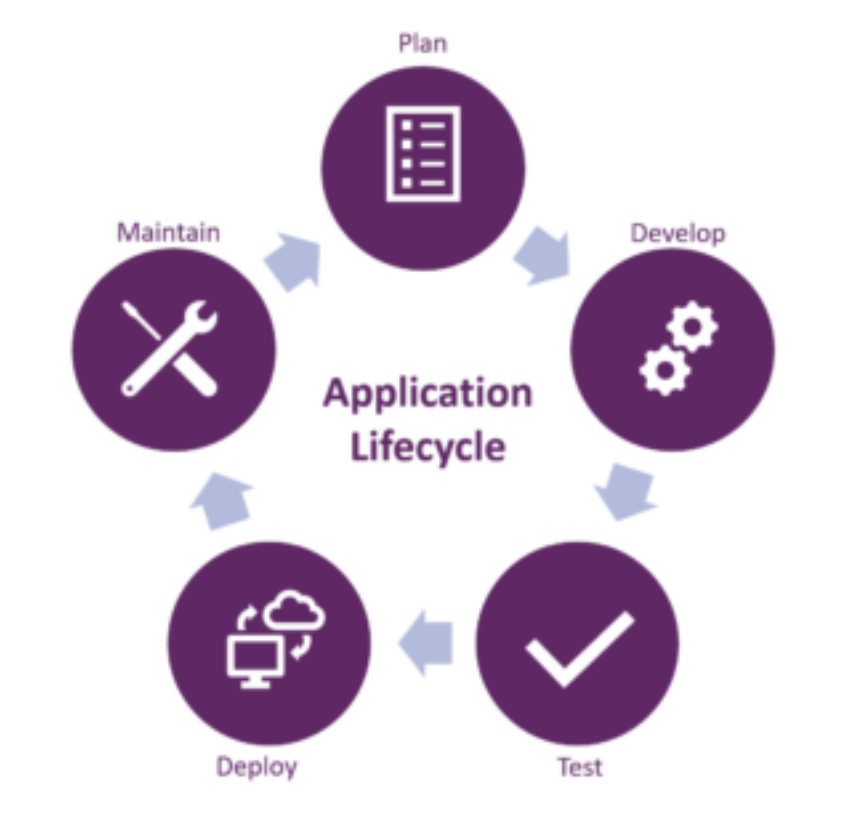
\includegraphics[scale = 0.3]{attachment/chapter_13/Scc026}
	\caption{Application Lifecyle} 
\end{figure}

Für \gls{ALM} steht im Kern
\begin{center}
	\textit{No code development} != \textit{No DevOps}
\end{center}

Die folgenden Unterkapitel greifen die Schwerpunkte des \gls{ALM} in \gls{PP} auf.

Mehr zu dem Thema unter \href{https://docs.microsoft.com/de-de/power-platform/alm/solution-concepts-alm#solution-publisher}{Solution Lebenszyklus}  
\subsection{Solution}
\subsubsection{Un- and Managed Solution}
Solutions sind Pakete, welche von einer oder mehreren Applikationen verwendet werden. Eine Solution dient als Transportmittel, welche alle relevanten Komponenten mindestens einer Applikation enthält. Eine Solution wird von einem \textit{Publisher} veröffentlicht und befindet sich in einer \Env. 

Was eine Solution enthalten kann, ist vielfältig. Von einem Data Model, den \gls{UI} Komponenten, Prozess Stritt und anderen relevanten Komponenten einer Applikation.
\begin{figure}[H]
	\centering
	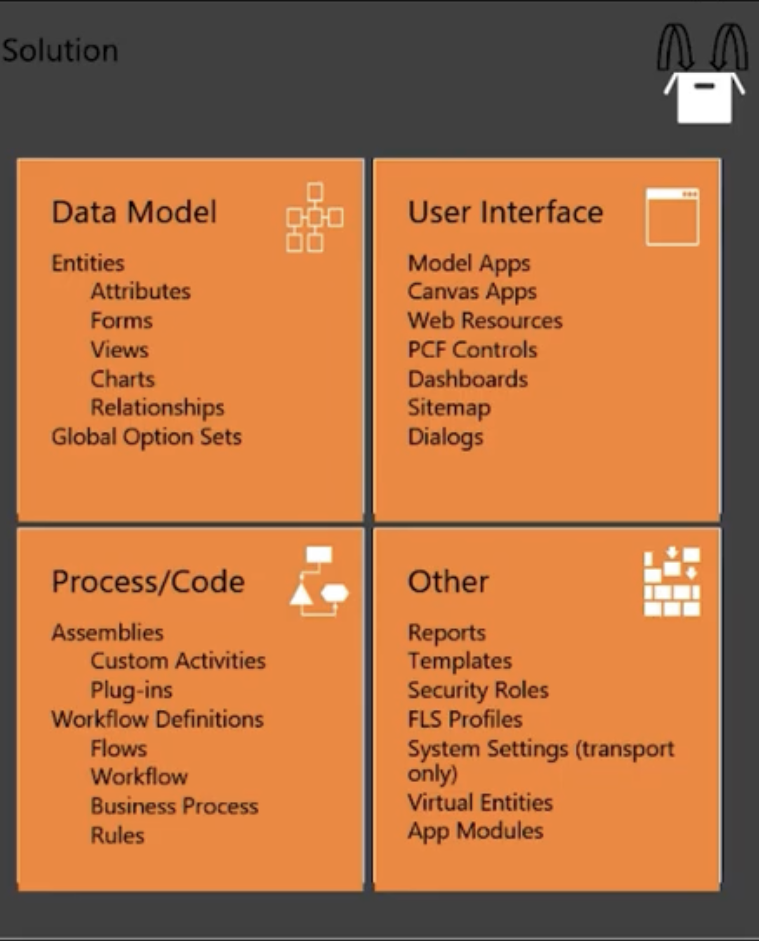
\includegraphics[scale = 0.3]{attachment/chapter_13/Scc028}
	\caption{Inhalte einer Solution} 
\end{figure}

Um Solutions zwischen \Envs zu transportiert wird die Export Funktion in der Web Applikation verwendet. Später wird gezeigt, wie dies über Azure funktioniert.
Wenn eine Solution in der Entwicklungsumgebung erstellt wird hat diese automatisch die Eigenschaft \textit{unmanaged}. Bei Export kann zwischen \textit{un-} und \textit{managed} ausgewählt werden. 

Eine \textit{unmanaged Solution} ist für die Weiterbearbeitung freigeschalten. Eine \textit{managed Solution} erlaubt eine Bearbeitung der Bestandteile in ihr nicht.
\begin{figure}[H]
	\centering
	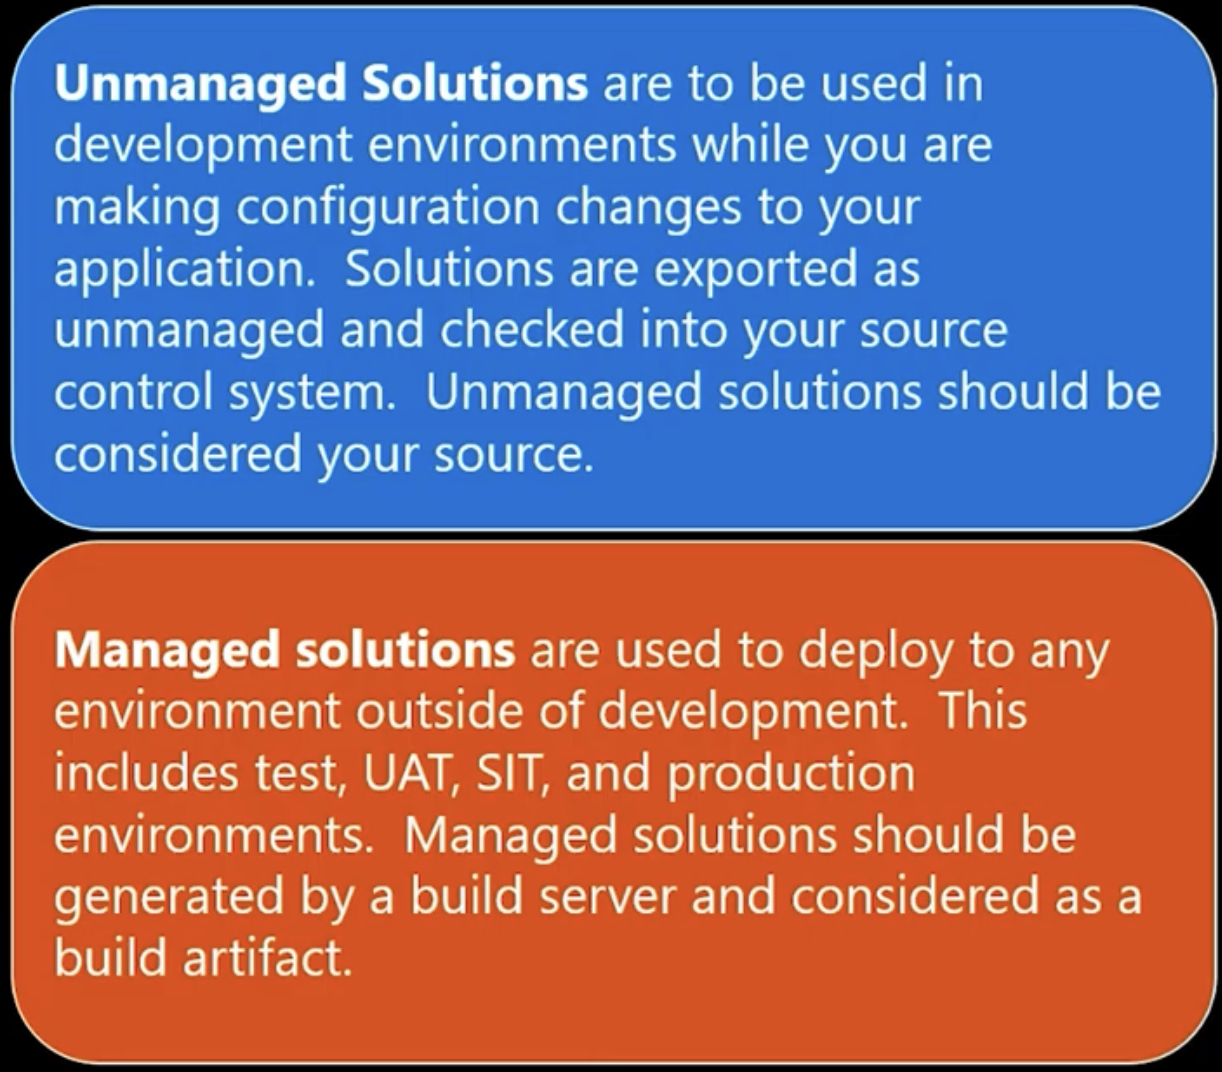
\includegraphics[scale = 0.3]{attachment/chapter_13/Scc029}
	\caption{Managed and Unmanaged Solution} 
\end{figure}

Im späteren Prozess wird gezeigt, wie ein unmanaged Solution in ein \gls{g_Git} Repository geladen wird und dort als \textit{Source of Truth} dient.
Eine \textit{managed Solution} wird als ein \gls{BuildArtifacts} verstanden und soll in nur in Test und Produktionsumgebungen überführt werden.

Wir eine Solution erstellt, wird die Versionnummer mit 1.0.0.0 festgelegt und ein Name sowie Publisher werden ausgewählt.
\begin{figure}[H]
	\centering
	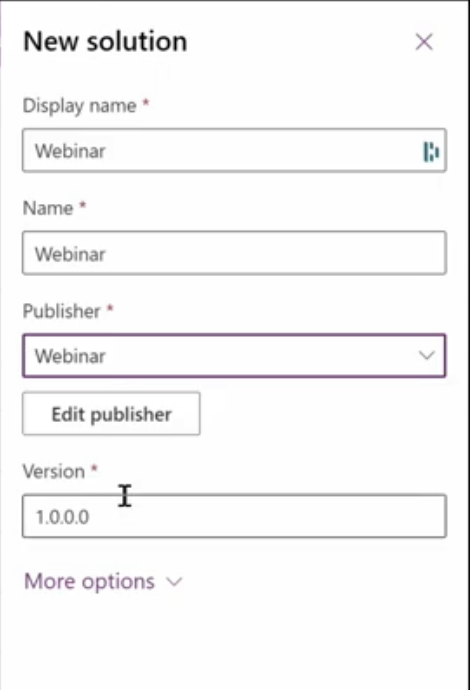
\includegraphics[scale = 0.3]{attachment/chapter_13/Scc030}
	\caption{Neu Solution} 
\end{figure}

Die Versionsnummer Logik ist <major>.<minor> ist für Kombinierungen von Patches oder größere Änderungen an der Solution. <build>.<revision> werden für Patches verwendet.


Die Eigenschaft, ob eine Solution managed oder unmanaged ist, wird mit dem Export einer Solution festgelegt.
\begin{figure}[H]
	\centering
	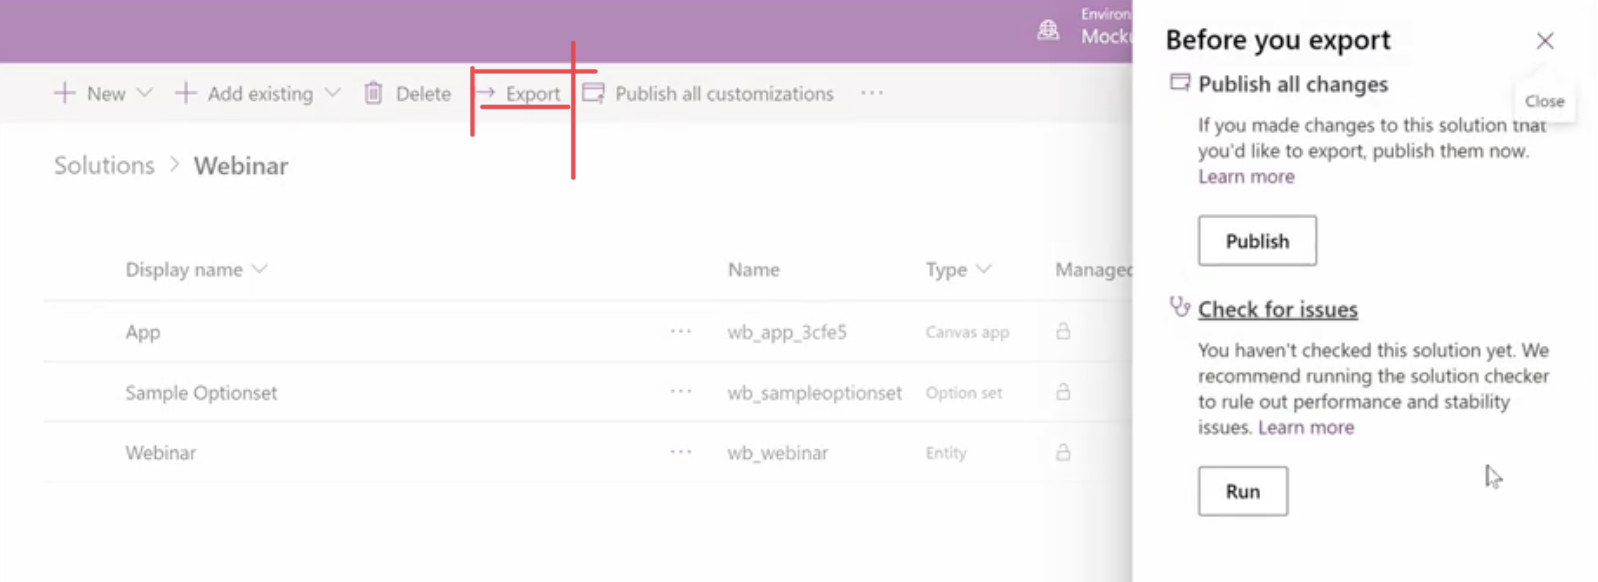
\includegraphics[scale = 0.3]{attachment/chapter_13/Scc032}
	\caption{Step 1 of Export} 
\end{figure}
\begin{figure}[H]
	\centering
	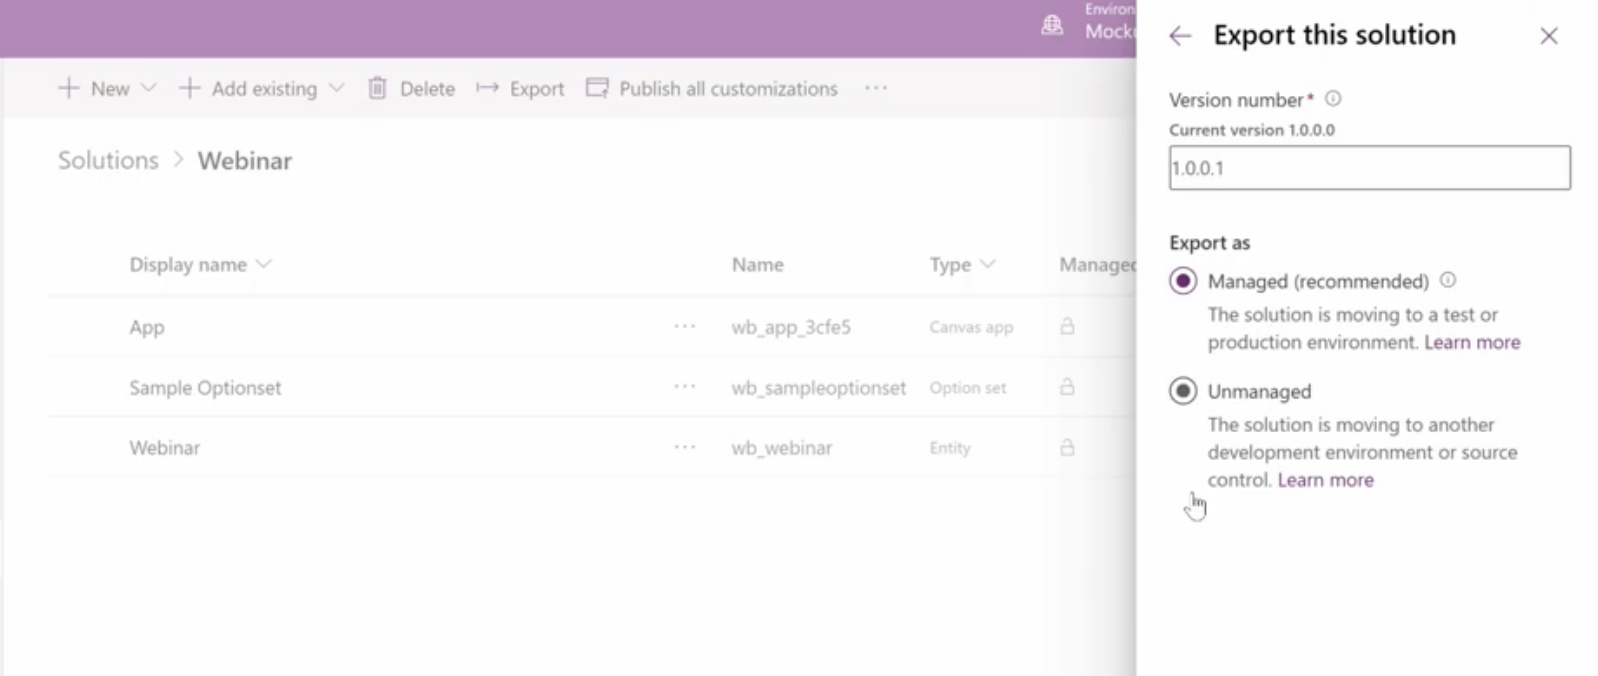
\includegraphics[scale = 0.3]{attachment/chapter_13/Scc033}
	\caption{Step 2 of Export} 
\end{figure}

\subsubsection{Update Solution through Layering}
\paragraph*{Clone a patch}
Die Patch Funktion bietet an, dass Komponenten ergänzt oder geändert werden. Löschen von Komponenten ist nicht möglich. Ebenso kann ein Patch nur angewandt werden, wenn es die gleiche <major>.<minor> Nummer hat. \\

In der Solution befindet sich eine \textit{Site Map}, eine \textit{Model-Driven App} und zwei \textit{Table}.
\begin{figure}[H]
	\centering
	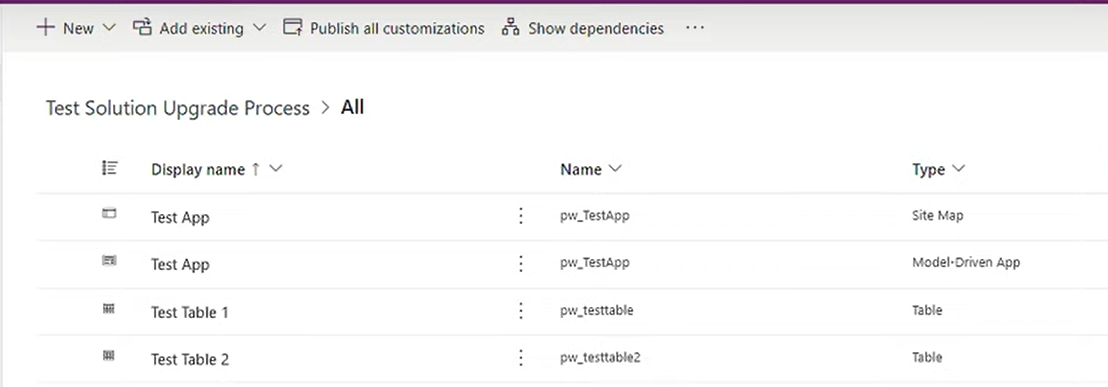
\includegraphics[scale = 0.3]{attachment/chapter_13/Scc034}
\end{figure}

In der Produktion zeigt die Test-App vier Einträge. Der vierte Eintrag ist \textit{Company Revenue}.  Dieser soll über ein \textit{Patch} geändert werden.
\begin{figure}[H]
	\centering
	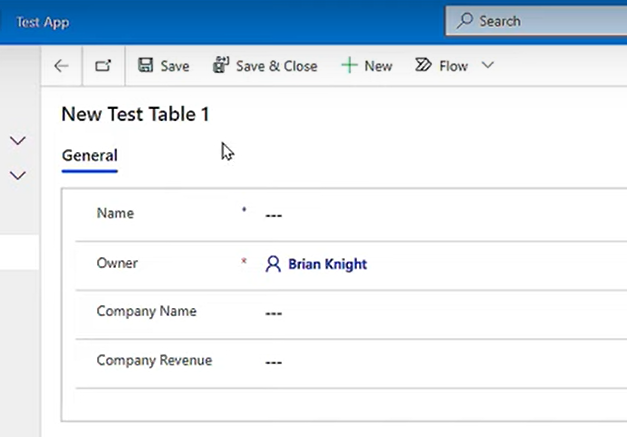
\includegraphics[scale = 0.3]{attachment/chapter_13/Scc035}
\end{figure}

In der Entwicklungsumgebung wird ein Solution von der Parent Solution \textit{Test Solution Upgrade Process} erstellt. Warum die Änderungen nicht direkt in der Solution getätigt wird, ist, dass noch weitere Änderungen vorgenommen wurden, welche noch nicht für die Produktion fertig sind.
\begin{figure}[H]
	\centering
	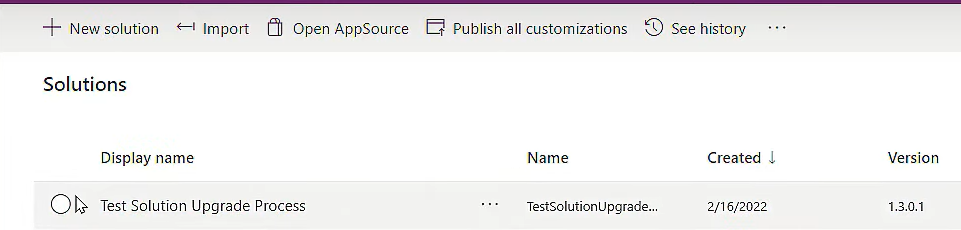
\includegraphics[scale = 0.3]{attachment/chapter_13/Scc036}
	\caption{Parent Solution}
\end{figure}
Mit dem Clone für den Patch
\begin{figure}[H]
	\centering
	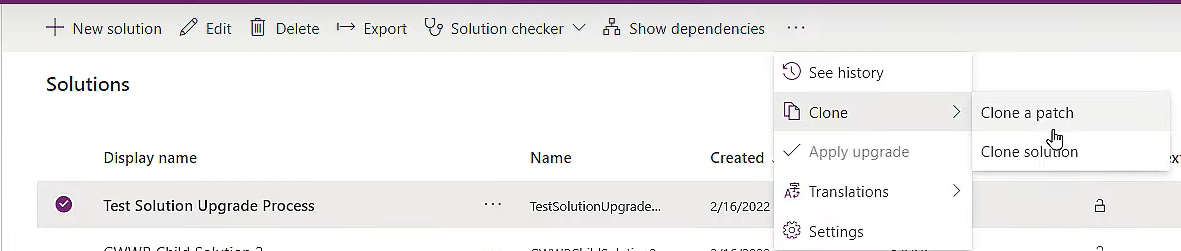
\includegraphics[scale = 0.3]{attachment/chapter_13/Scc037}
	\caption{Clone a patch}
\end{figure}
\begin{figure}[H]
	\centering
	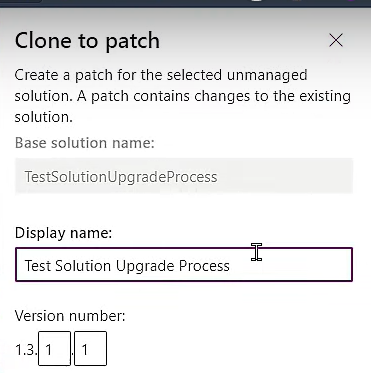
\includegraphics[scale = 0.3]{attachment/chapter_13/Scc038}
\end{figure}
kann eine neuer Displayname erstellt werden und eine Inkrementierung für die Versionsnummer für <build>.<revision> erstellt werden.\\
Das Result ist eine neue Solution mit 1.3.1.1 
\begin{figure}[H]
	\centering
	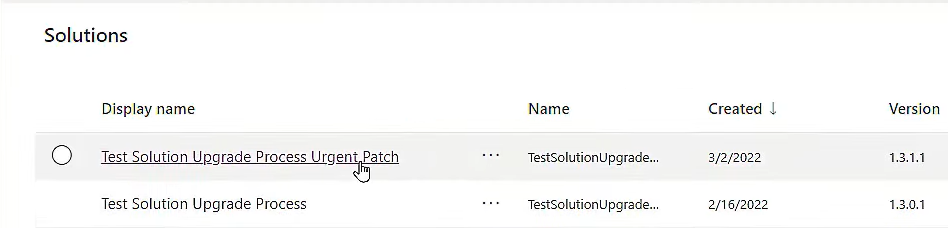
\includegraphics[scale = 0.3]{attachment/chapter_13/Scc039}
\end{figure}
Diese ist jedoch leer
\begin{figure}[H]
	\centering
	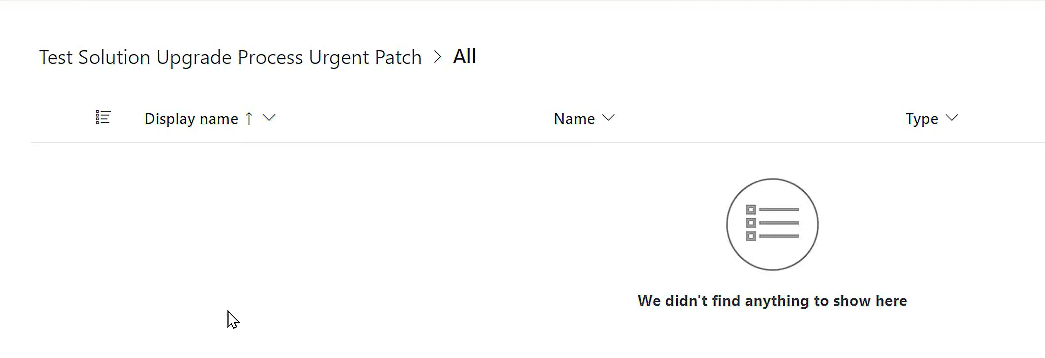
\includegraphics[scale = 0.3]{attachment/chapter_13/Scc040}
\end{figure}
Es enthält das Schema der Parent Solution. Somit kann \textit{Test Table 1} aus dem Dataverse hinzugefügt werden. Dies gilt für alle anderen Komponenten einer Solution ebenfalls.
\begin{figure}[H]
	\centering
	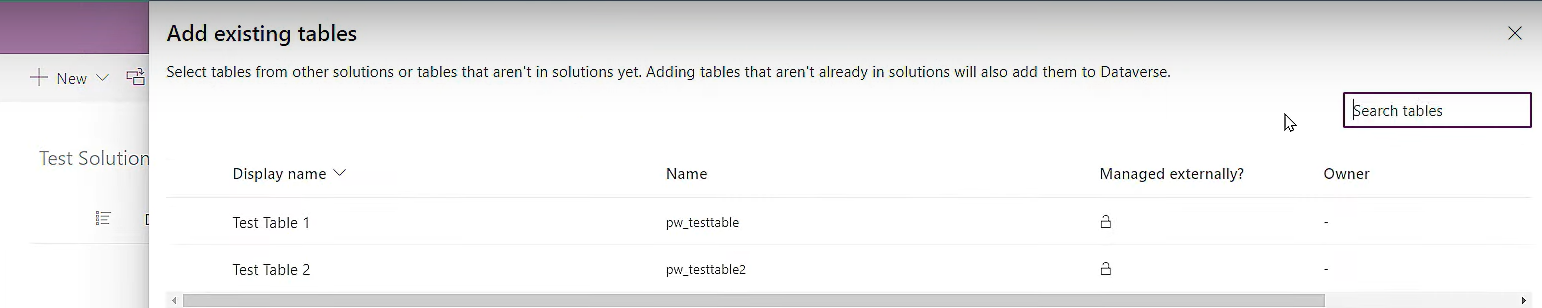
\includegraphics[scale = 0.3]{attachment/chapter_13/Scc041}
\end{figure}
Dies ist jetzt in der Solution zu finden.
\begin{figure}[H]
	\centering
	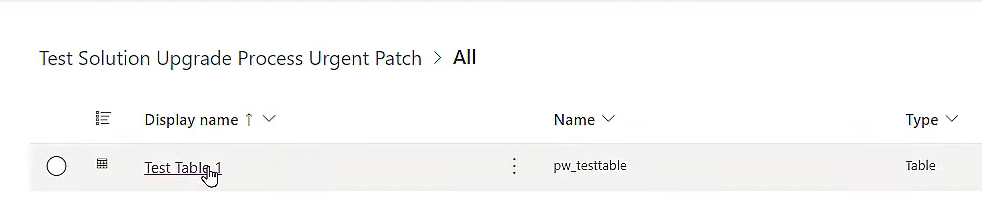
\includegraphics[scale = 0.3]{attachment/chapter_13/Scc042}
\end{figure}

Das Ziel war, die Spalte \textit{Company Revenue} zu ändern.
\begin{figure}[H]
	\centering
	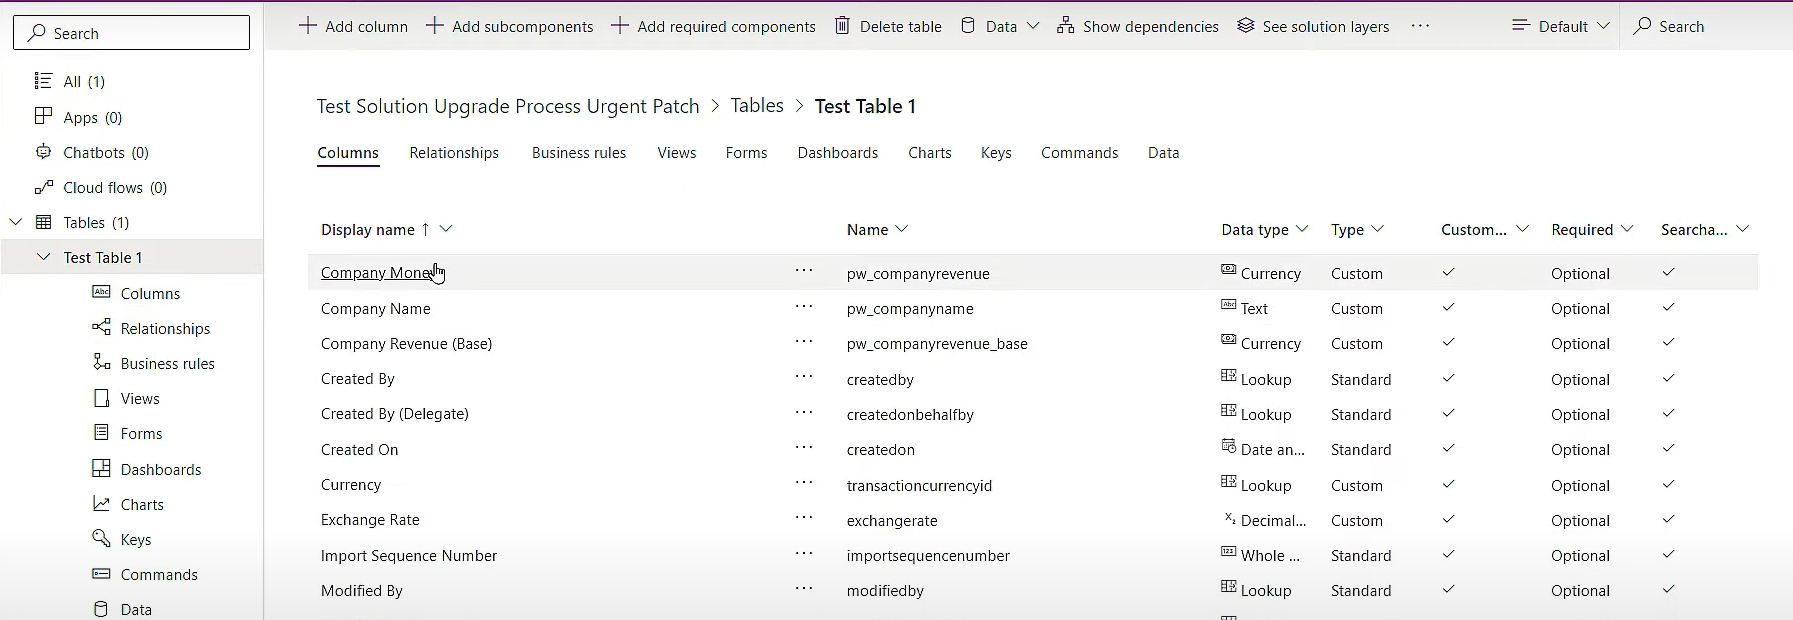
\includegraphics[scale = 0.3]{attachment/chapter_13/Scc043}
\end{figure}
In der Form Ansicht ist der Wert der Spalte zu finden.
\begin{figure}[H]
	\centering
	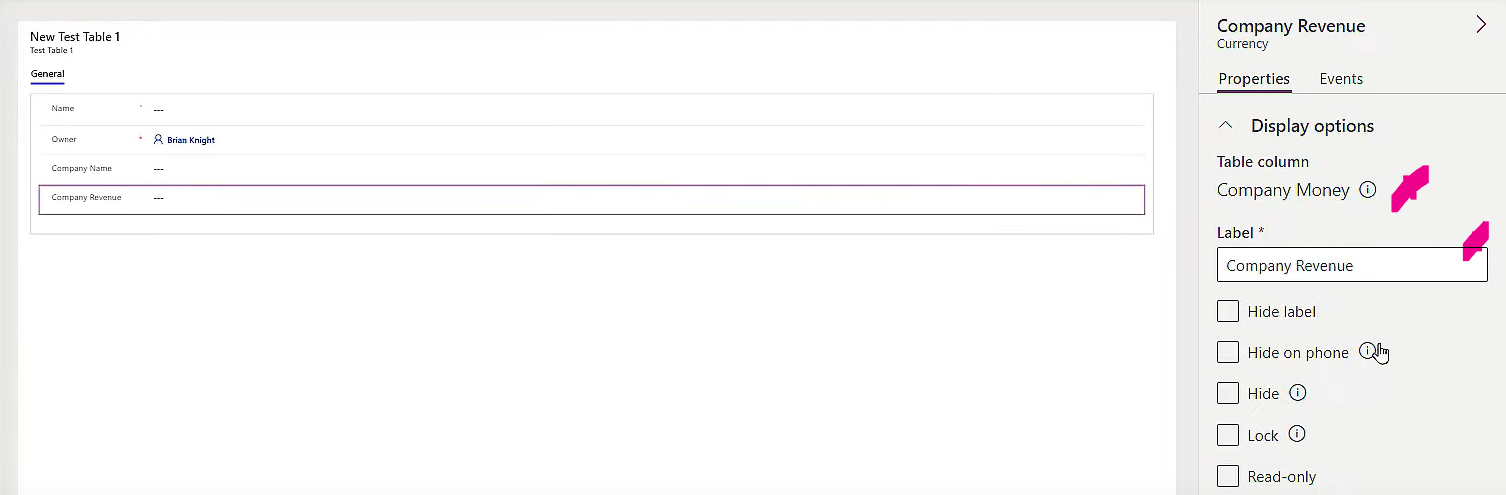
\includegraphics[scale = 0.3]{attachment/chapter_13/Scc044}
\end{figure}
Dieser wird von \textit{Company Revenue} zu \textit{Company Money} geändert. Die App wird daraufhin gespeichert und die Solution exportiert mit dem Inkrement 1.3.1.2
\begin{figure}[H]
	\centering
	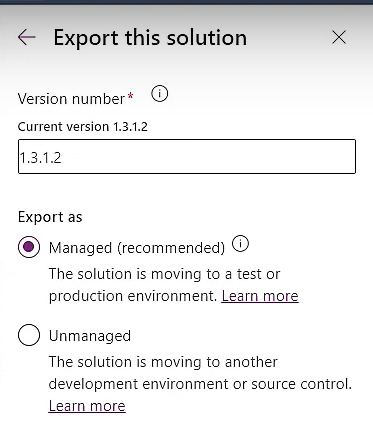
\includegraphics[scale = 0.3]{attachment/chapter_13/Scc045}
\end{figure}

In der Produktion oder Testumgebung wird dieser Patch importiert.
\begin{figure}[H]
	\centering
	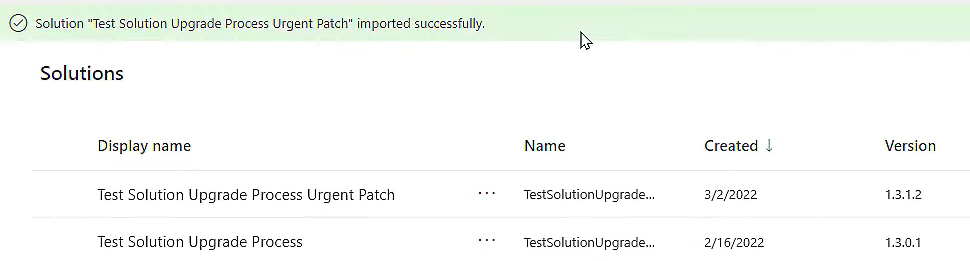
\includegraphics[scale = 0.3]{attachment/chapter_13/Scc046}
\end{figure}


Die App in der Produktion oder Testumgebung zeigt jetzt die Änderungen mit dem Spaltennamen \textit{Company Money}.
\begin{figure}[H]
	\centering
	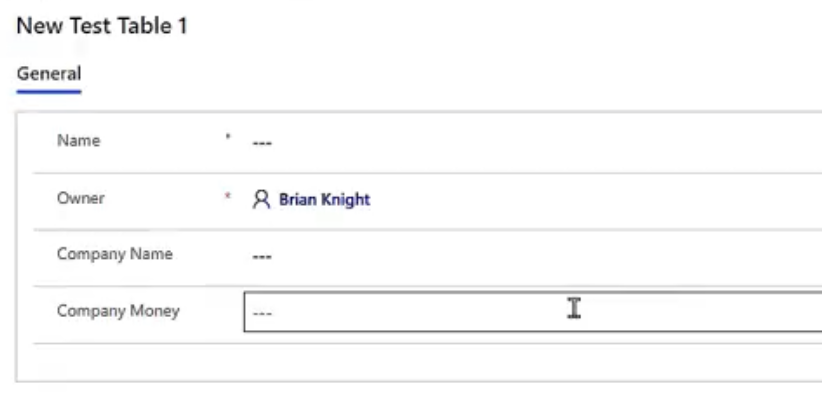
\includegraphics[scale = 0.3]{attachment/chapter_13/Scc047}
\end{figure}


\paragraph{Clone Solution - Merging}

Wenn die komplette Entwicklung abgeschlossen ist in \textit{Test Solution Upgrade Process} kann mit \textit{Clone Solution} ein \textit{Merge} zwischen der \textit{Parent Solution} und der einen oder mehreren Patches angestoßen werden. Dafür wird unter der Parent Solution die Option \textit{Clone Solution} ausgewählt.

\begin{figure}[H]
	\centering
	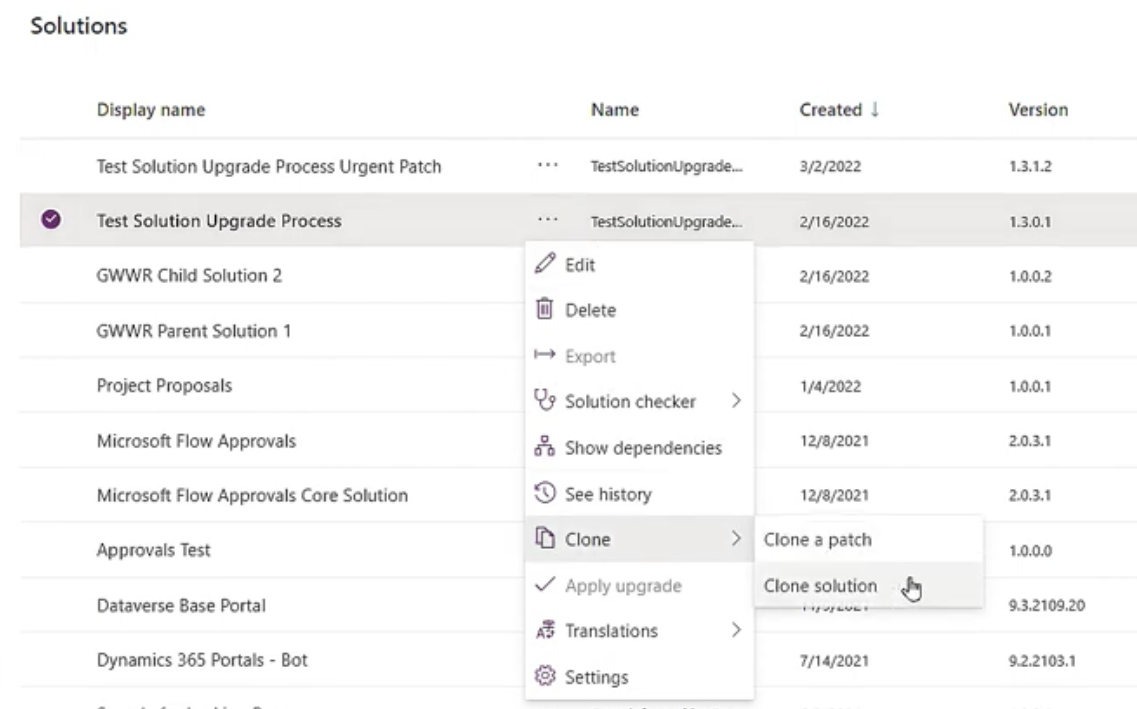
\includegraphics[scale = 0.3]{attachment/chapter_13/Scc048}
	\caption{Vor dem Merge}
	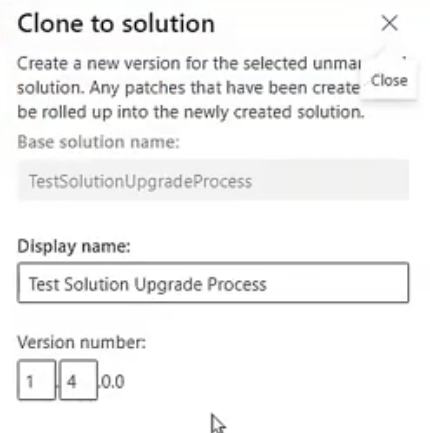
\includegraphics[scale = 0.3]{attachment/chapter_13/Scc049}
	\caption{Für dies Version kann nur <major>.<minor> ausgewählt werden.}
	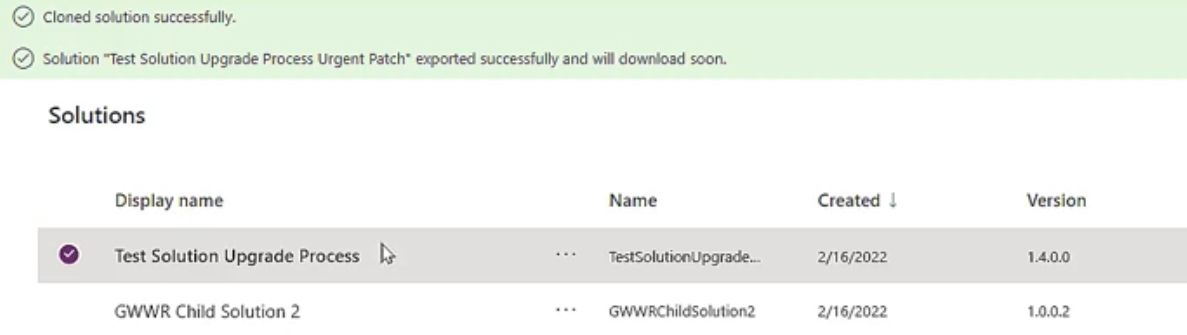
\includegraphics[scale = 0.3]{attachment/chapter_13/Scc050}
	\caption{Nach dem Merge}
\end{figure}

Nach dem Merge existiert nur noch eine Solution, welche mit der Versionsnummer 1.4.0.0 versehen ist.

Angenommen in der Solution wird in der Entwicklungsumgebung noch weitere Änderungen vorgenommen, so werden diese ebenfalls mit integriert. Wird die gemergte Solution exportiert, wird diese mit 1.4.0.1 in die Produktions- oder Testumgebung importiet

\begin{figure}[H]
	\centering
	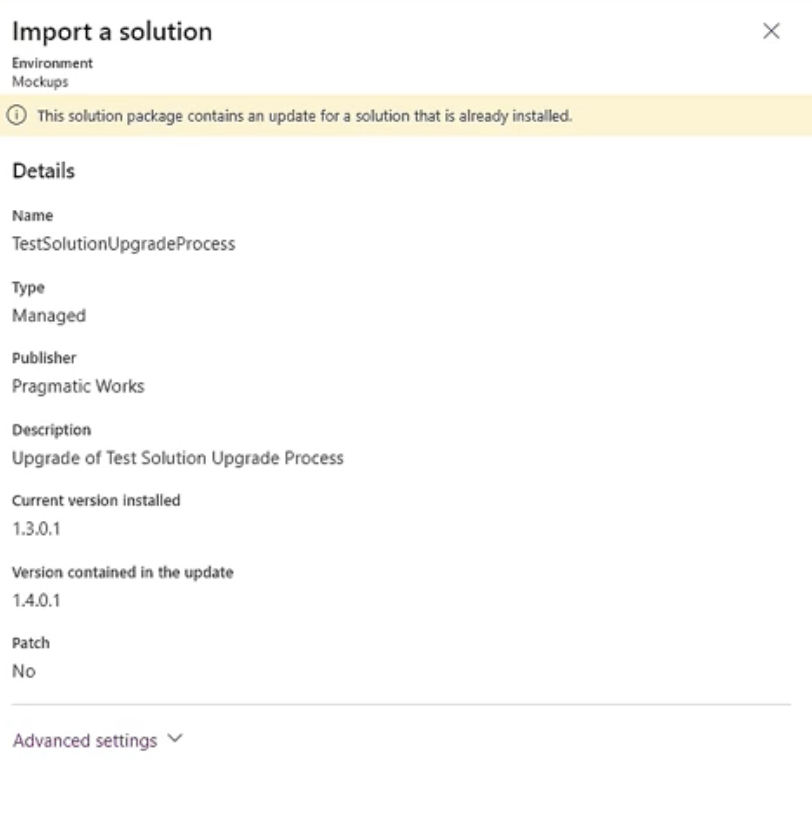
\includegraphics[scale = 0.3]{attachment/chapter_13/Scc051}
\end{figure}

In der Zielumgebung verschwinden die Patch Solution ebenfalls, sodass nur noch die Solution mit der Versionsnummer 1.4.0.1 überbleibt.

\paragraph{Layering}
Die verschiedenen Solution werden in Dataverse in der Zielumgebung installiert, Updates, Upgrades oder Patches werden hier nach einander geschalten. Der Aufbau ist, dass ungemanagete Solution als oberste Schicht angelegt werden, danach kommen die gemanageten Lösungen, welche gemäß ihrer Versionsnummer gestappelt werden. 

Mehr zu dem Thema und dem Verhalten verschiedenster Merge Probleme unter 

\href{https://benediktbergmann.eu/2022/01/18/dataverse-solutions-explained/}{Updates und Layering}, \href{}{} 

\paragraph{Upgrade or Update}
Der Unterschied ist nur, dass bei einem Upgrade, die Komponenten, welche nicht in der Zielsolutionumgebung vorhanden sind gelöscht werden. Bei einen Update bleiben diese erhalten.
\begin{figure}[H]
	\centering
	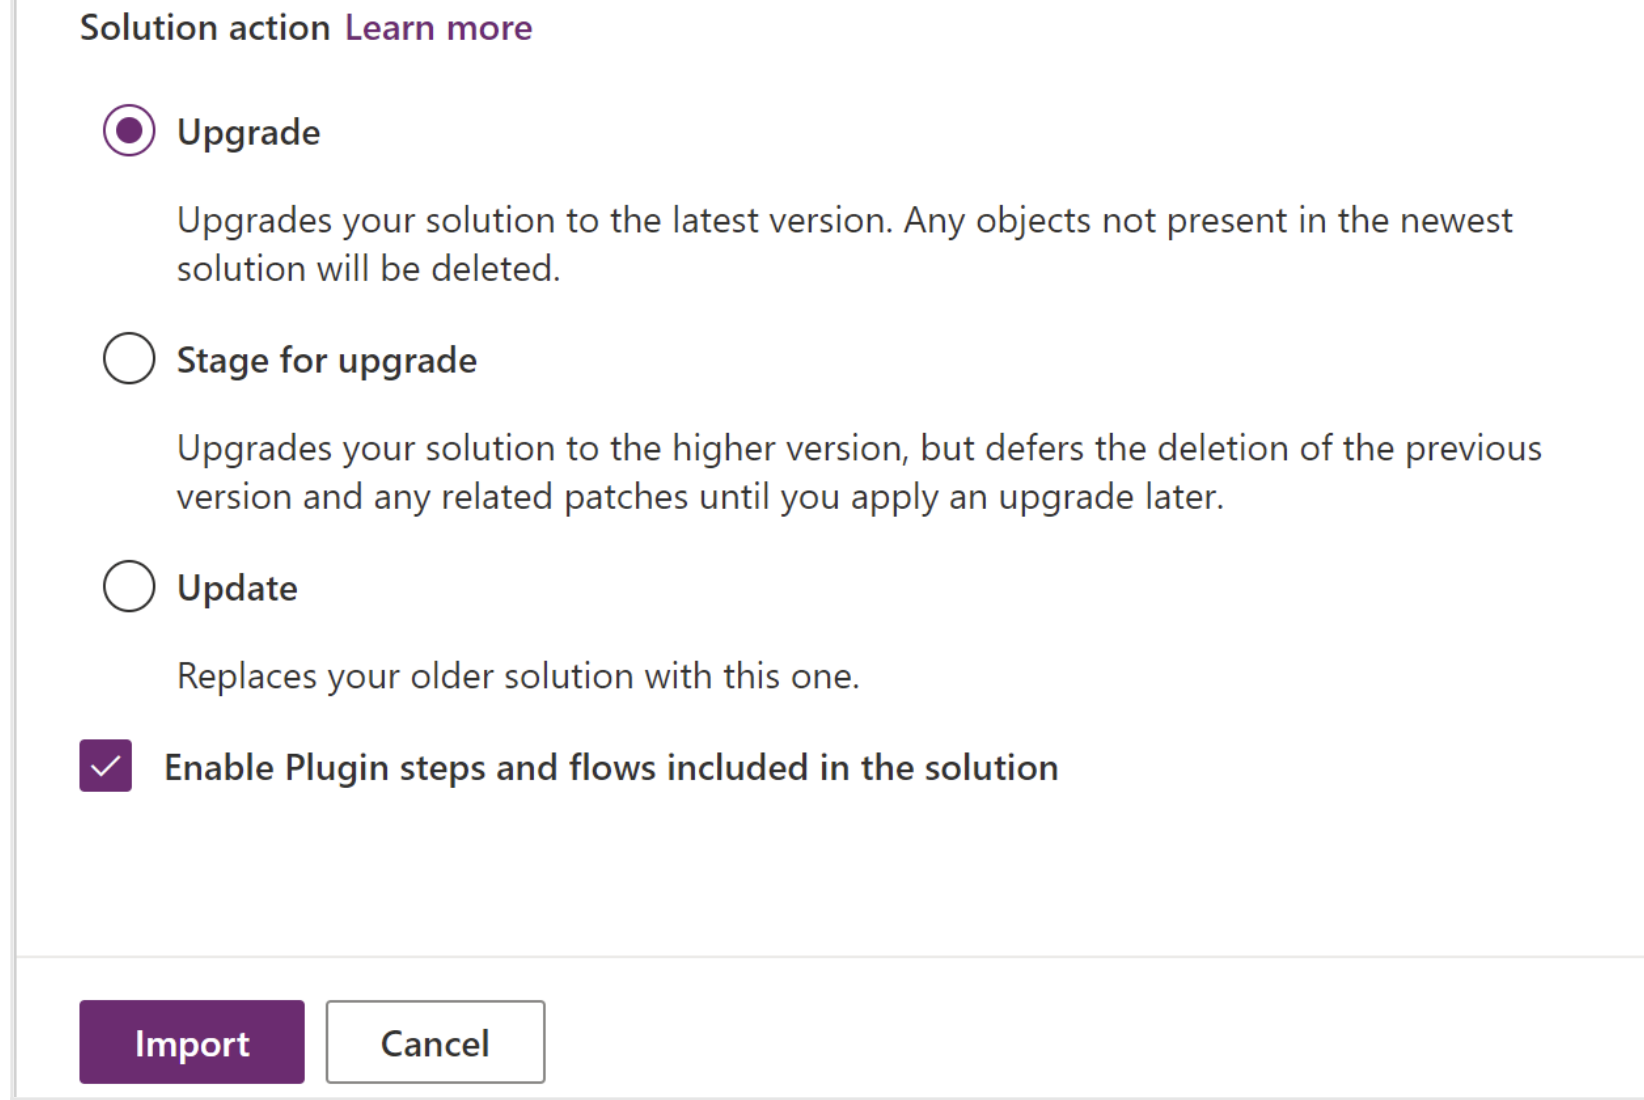
\includegraphics[scale = 0.3]{attachment/chapter_13/Scc053} 
\end{figure}


\subsection{ALM Strategy}
Die hängt davon ab, wie groß und verknüpft die Applikationen mit einander sind.

Thema Referenzen: \href{https://benediktbergmann.eu/2022/01/18/dataverse-solutions-explained/}{Split Solution}, \href{https://docs.microsoft.com/en-us/powerapps/maker/data-platform/solution-layers}{Solution Layer}


\paragraph{Azure - Source of Truth - Repo}
Die Allgemeinen Vorteile einer Zentralen Verwaltung des Quell-Codes sind:
\begin{itemize}
	\item Depoly Hotfixes, während noch an der nächsten Version gearbeitet wird. Aus dem Repository werden die Solution gespeist.
	\item Mehrer Entwickler können an einer App bauen, welche über den \gls{ALM} Prozess im Quell Verzeichnis zusammengefügt werden. Von dort aus, wird der Merge Prozess gestartet und die Solution gebildet.
\end{itemize}

Das Ziel ist dabei nicht eine Historie der Zip-Dateipacketen, sondern einer Verwaltung der einzelnen Dateien. Azure Pipeline bietet \textit{\textbf{Solution Packager}}, welche die Zip-Files entpackt und in den Bestandteile abspeichert. \textit{\textbf{Solution Packager}} kontrolliert Konfiguration und Performance Parameter. Zum Beispiel wird kontrolliert, dass die alle Bestandteile in einer Solution des gleichen Publisher stammen, somit dies bewegt werden können.


% TODO: Solution Checker

\section{Building}
\subsection{Open Topics}
\paragraph{Connector}
Diese ins API-Wrapper, welche die Zugangsdaten für die \gls{API} regeln. Diese können in einer Solution separat hinterlegt werden, siehe \href{https://docs.microsoft.com/en-us/power-apps/maker/data-platform/create-connection-reference}{Create Connectionreference}  

\paragraph{Developer Terminology} 
Unter 
\href{https://docs.microsoft.com/en-us/powerapps/developer/data-platform/understand-terminology}{Terminology}
 können die verschieden Bezeichnungen für Tabellen, Reihen, Spalten und weiteres in den verschiedensten Umgebungen zu sehen sein.
 \begin{figure}[H]
	\centering
	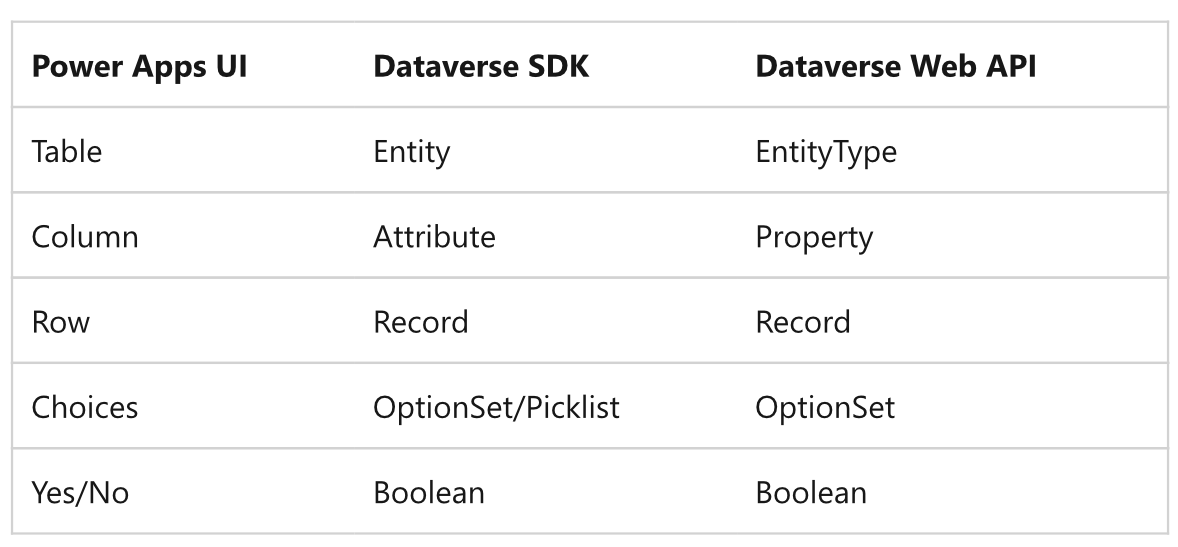
\includegraphics[scale = 0.3]{attachment/chapter_13/Scc052}
	\caption{Developer Terminlogy} 
\end{figure}

\paragraph{Fragestellungen}
\begin{enumerate}
	\item Die Splitting Solution \gls{ALM} Strategy ist nicht klar, wie Komponenten aus einer Solution von einer App in einer andern Solution aufgegriffen werden können.
	\item Test von Layering. Im direkten ALM Prozess der DB, die Upgrade Funktion testen.
	\item \Env Varialben: Was passiert, wenn man nicht alle Komponeten (Add required Component) mit in die Solution genommen hat?
\end{enumerate}

\subsection{Environment Variablen}
\paragraph{SharePoint Connector in Canvas App}
Siehe \href{https://docs.microsoft.com/en-us/powerapps/maker/data-platform/environmentvariables#how-do-they-work}{Environment Variables}

Um Connection Referenzen gleich mit einer Enviromnent Variablen zu verbinden, wird in der App unter Einstellung die Option: Erstelle automatische eine Envirorment Variablen angeklickt.

\begin{figure}[H]
	\centering
	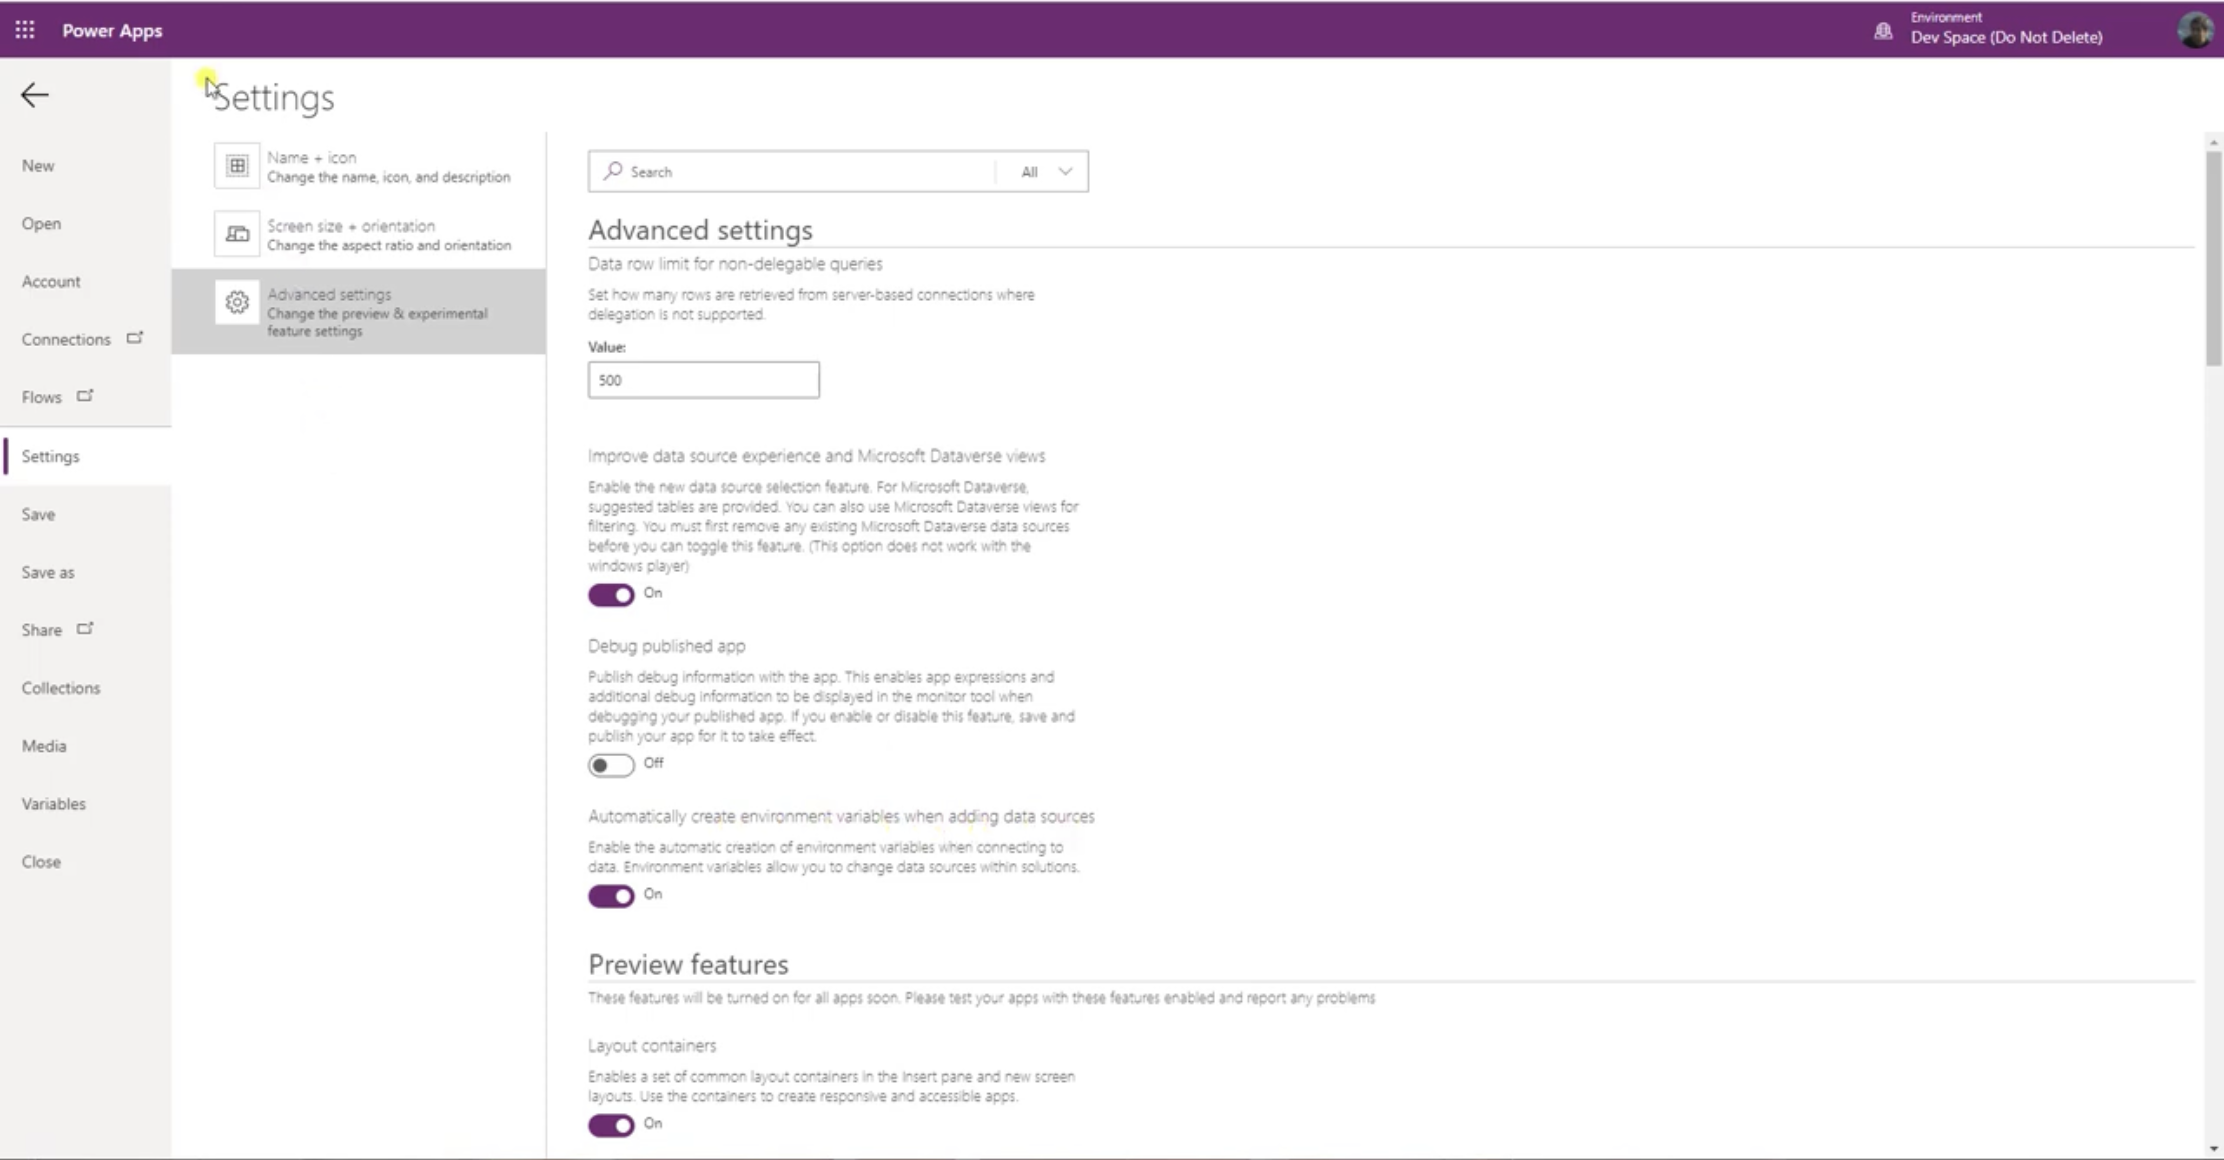
\includegraphics[scale = 0.3]{attachment/chapter_13/Scc054}
\end{figure}

Wenn sich mit dem SharePoint Connector verbunden wird, kann unter der Referenz eine spezifische Liste ausgewählt werden. Unter Advance kann, wenn vorhanden, eine \Env Variable auswählen werden.

\begin{figure}[H]
	\centering
	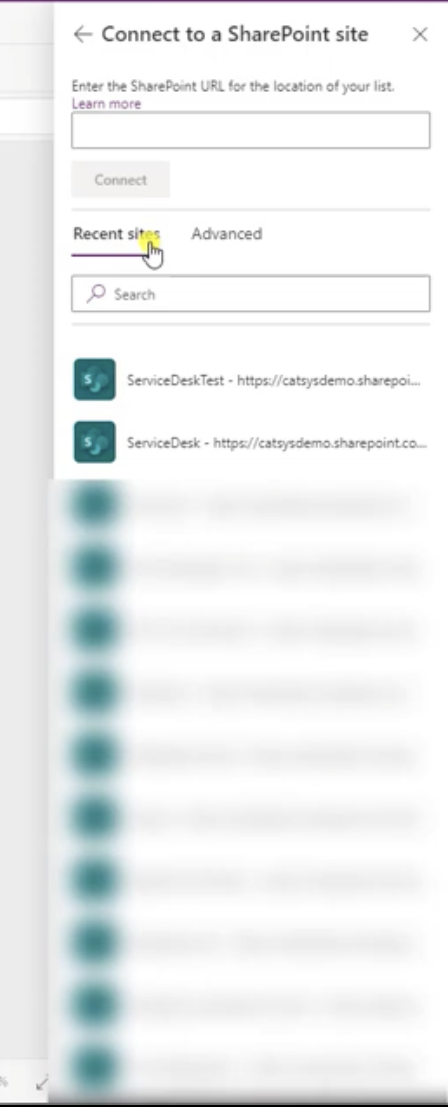
\includegraphics[scale = 0.3]{attachment/chapter_13/Scc055}
\end{figure}

Wenn die Verbindung angelegt ist, wird angezeigt, dass eine \Env Variable erstellt wurde.

\begin{figure}[H]
	\centering
	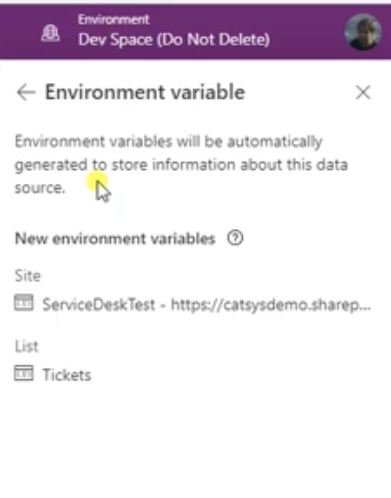
\includegraphics[scale = 0.3]{attachment/chapter_13/Scc056}
\end{figure}

In der Solution sind zwei Variablen für den SharePoint Konektor angelegt worden.

\begin{figure}[H]
	\centering
	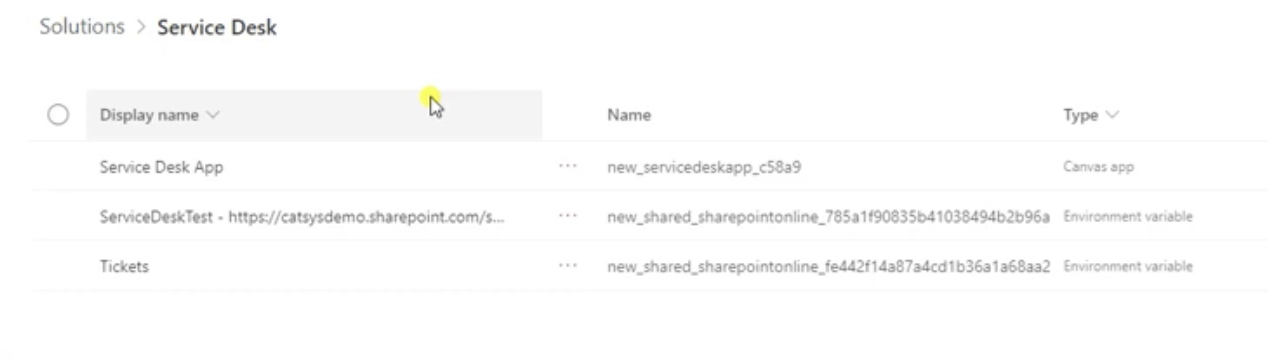
\includegraphics[scale = 0.3]{attachment/chapter_13/Scc058}
\end{figure}

Die erste \Env Variablen ist für den Ort, in welcher die Liste liegt. Die zweite für den Namen der Liste.

\paragraph{Flow}
Soll ein Nutzer informiert werden, wenn eine neues Element erstellt wird, wird ein Flow angelegt. Dieser verweißt auf die SharePoint Seite. Anstatt die Adresse und Namen für die Liste zu hinterlegen,

\begin{figure}[H]
	\centering
	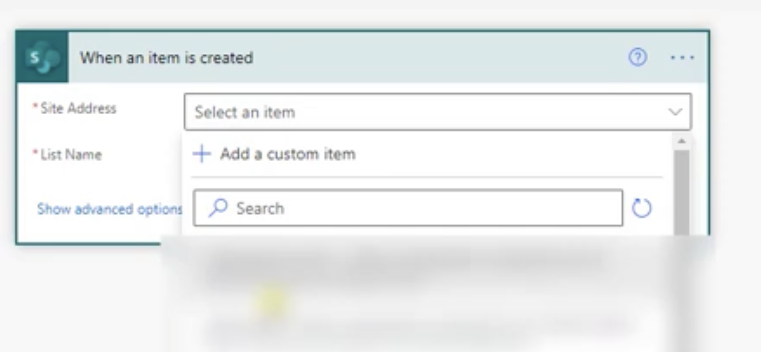
\includegraphics[scale = 0.3]{attachment/chapter_13/Scc057}
\end{figure}

wird auf \textit{Add customm item} geklickt, kann unter Parameters, die hinterlegten Variablen ausgewählt werden.

\begin{figure}[H]
	\centering
	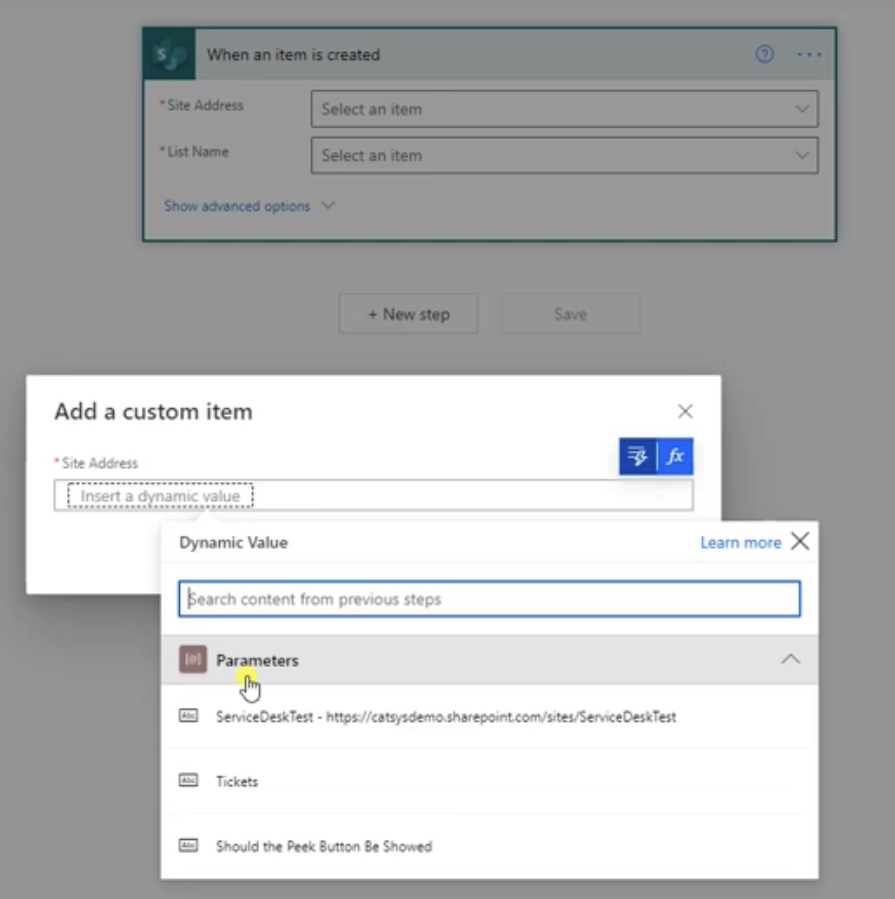
\includegraphics[scale = 0.3]{attachment/chapter_13/Scc059}
\end{figure}

\paragraph{Solution Required Connectoren}
Um sicherzustellen, dass alle Konnektoren in der Solution liegen, wird auf das Element, in dem Fall Canvas Apps und den Flow, unter \textit{Add required Componente}

\begin{figure}[H]
	\centering
	\includegraphics[scale = 0.3]{attachment/chapter_13/Scc060}
\end{figure}

geklickt. Für den Flow wird der Outlook und SharePoint Connecktor hinzugefügt.

\begin{figure}[H]
	\centering
	\includegraphics[scale = 0.3]{attachment/chapter_13/Scc061}
\end{figure}

\paragraph{Delete Current Selection}
Die aktuelle Auswahl der \Env Variable wird vor dem Export gelöscht. Dabei besteht die Möglichkeit den hinterlegten Wert aus der Solution oder aus der \Env zu löschen.

\begin{figure}[H]
	\centering
	\includegraphics[scale = 0.3]{attachment/chapter_13/Scc062}
\end{figure}

\paragraph{Import Solution}
Wenn die Solution in die Test oder Produktions \Env geladen wird, wird nach den Connections References gefragt.

\begin{figure}[H]
	\centering
	\includegraphics[scale = 0.3]{attachment/chapter_13/Scc063}
\end{figure}

Im Folgenden wird nach den \Env Variablen gefragt:

\begin{figure}[H]
	\centering
	\includegraphics[scale = 0.3]{attachment/chapter_13/Scc064}
\end{figure}

Zum Ende, wenn die Application gestartet wird, wird nach dem Zertifikat für gewissen Konnektoren gefragt.

\begin{figure}[H]
	\centering
	\includegraphics[scale = 0.3]{attachment/chapter_13/Scc065}
\end{figure}